%usenix 2023
\documentclass[letterpaper,twocolumn,10pt]{article}
\usepackage{usenix-2020-09}



\usepackage[small]{titlesec}
% to be able to draw some self-contained figs
%\usepackage{tikz}
\usepackage{amsmath}
\usepackage{bm}

% inlined bib file
\usepackage{filecontents}

\usepackage{wasysym}


\usepackage{lipsum,cuted}
\usepackage{float}
\usepackage{caption}


\pagestyle{plain}


\usepackage{graphicx}
\usepackage{verbatim}
\usepackage{caption}
%

%\usepackage{algpseudocode}
\usepackage{amsmath,amssymb,amsthm}

%\usepackage{graphicx}
%\usepackage{geometry}
\usepackage{subfigure}
\usepackage{url}
\usepackage{multirow}
\usepackage{listings}
\usepackage{cite}
\usepackage{array}
\usepackage{enumerate}
\usepackage{booktabs}
\usepackage{color}
\usepackage{xcolor}
\usepackage{soul}
\usepackage{multicol}
%\usepackage{algcompatible}
%\usepackage[compatible]{algpseudocode}


\renewcommand{\thefootnote}{*}

\newcommand\usso{\textsf{UPPRESSO}}
\newcommand\dyu{{DYU}}

\newtheorem{thm}{\textsc{Theorem}}
\newtheorem{lemma}{\textsc{Lemma}}
%\newtheorem{theorem}{Theorem}
\newtheorem{definition}{\textsc{Definition}}
%\newtheorem{lemma}{Lemma}





\definecolor{Blue}{RGB}{0,0,255}
\newcommand{\newc} {\color{Blue}}
\newcommand{\oldc} {\color{black}}

% correct bad hyphenation here
\hyphenation{target-Origin js-rsa-sign op-tical net-works semi-conduc-tor}

\begin{document}
\date{}
\pagenumbering{arabic}
%\title{\Large \bf \usso: Untraceable and Unlinkable Privacy-PREserving\\Single Sign-On Services\footnotemark[1]}
\title{\Large \bf \usso: Untraceable and Unlinkable Privacy-PREserving\\Single Sign-On Services}


% Chengqian Guo, Jingqiang Lin, Quanwei Cai, Fengjun Li, Wentian Zhu, Wei Wang, Jiwu Jing, Qiongxiao Wang, Bin Zhao

%\author{
%{\rm Chengqian Guo$^{\sharp\nabla}$, \ \ Jingqiang Lin$^{\ddag}$, \ \ Quanwei Cai$^{\P}$, \ \ Fengjun Li$^{\S}$, \ \ Wentian Zhu$^{\ddag}$, \ \ Wei Wang$^{\nabla}$,}\\
%{\rm Jiwu Jing$^{\diamondsuit}$, \ \ Qiongxiao Wang$^{\nabla}$, \ \ Bin Zhao$^{\triangle}$}\\
%$\sharp$ Shenyang Aircraft Design \& Research Institute, China\\
%$\ddag$ School of Cyber Security, University of Science and Technology of China\\
%$\P$ Beijing Zitiao Network Technology Co., Ltd, China\\
%$\S$  Department of Electrical Engineering \& Computer Science, the University of Kansas, USA\\
%${\diamondsuit}$ School of Computer Science \& Technology, University of Chinese Academy of Sciences\\
%$\nabla$ Institute of Information Engineering, CAS\ \ \ \ \ \ \ \ \ \ \ \ \ \ \ \ \ \ \ \ \ \ \ 
%$\triangle$ JD.com Silicon Valley R\&D Center, USA}



\maketitle
\begin{abstract}
Single sign-on (SSO) allows a user to maintain only the credential at an identity provider (IdP) to log into multiple relying parties (RPs).
However, SSO introduces privacy threats, as ({\em a}) a curious IdP could potentially track a user's visits to all RPs, and ({\em b}) colluding RPs could learn a user's online profile by linking her identities across these RPs.
This paper presents a privacy-preserving SSO protocol, called \usso, to protect an honest user's online profile against (\emph{a}) an honest-but-curious IdP and (\emph{b}) malicious RPs and users who could collude.
\usso\ proposes an identity-transformation approach to generate untraceable \emph{ephemeral pseudo-identities} for an RP and a user (denoted as $PID_{RP}$ and $PID_U$, respectively) from which the target RP derives a \emph{permanent account} for the user (denoted as $Acct$), while the transformations provide unlinkability.
This approach protects the unique identities of the user and the RPs that she requests to log into while working compatibly with SSO services and satisfying all the security requirements.
Compared with existing SSO protocols, \usso\ is among the first to prevent both types of privacy threats. Compared with existing privacy-preserving identity federation schemes, \usso\ supports all the desired SSO features while providing sufficient privacy protections.
% \usso\ proposes a novel identity-transformation approach. In each SSO login, an \emph{ephemeral pseudo-identity} of an RP, denoted as $PID_{RP}$, is negotiated between a user and the RP. $PID_{RP}$ is sent to the IdP and designated in the identity token, so that the IdP is not aware of the visited RP.
% The IdP then uses $PID_{RP}$ to transform the user's permanent identity $ID_U$, into an ephemeral user pseudo-identity $PID_U$, in the token.
% On receiving the identity token, %%%% the RP just waits for it.
% the RP transforms $PID_U$ into a \emph{permanent account} of the user, denoted as $Acct$. Given a user, the account at each RP is unique and different from $ID_U$, %%%% for different users, the accounts may be the same.
%so colluding RPs cannot link a user's identities across RPs.
We have built a prototype of \usso\ on top of MITREid Connect, an open-source SSO system. The extensive evaluations show that it fulfills the security and privacy requirements of SSO
while introducing reasonable overheads.
\end{abstract}

%\begin{IEEEkeywords}
%Single sign-on, security, privacy. %, trace, linkage
%\end{IEEEkeywords}

%\footnotetext[1]{Chengqian Guo participated in this work since his PhD study in Institute of Information Engineering, Chinese Academy of Sciences (CAS).}

\setcounter{footnote}{0}
\renewcommand{\thefootnote}{\arabic{footnote}}

\section{Introduction}
\label{sec:intro}
Single sign-on (SSO) protocols such as OpenID Connect (OIDC) \cite{OpenIDConnect}, OAuth 2.0 \cite{rfc6749}, and SAML \cite{SAML, SAMLIdentifier}, are widely deployed for identity management and authentication.
SSO allows a user to log into a website,
 known as the \emph{relying party} (RP), using her account registered at a trusted web service, known as the \emph{identity provider} (IdP).
An RP delegates user identification and authentication to the IdP, which issues an \emph{identity token} (such as ``id token'' in OIDC and ``identity assertion'' in SAML) for a user to visit the RP.
For instance, in an OIDC system, the user sends a login request to an RP,
which constructs an identity-token request with its identity (denoted as $ID_{RP}$) and redirects it to a trusted IdP. After authenticating the user, the IdP issues an identity token that binds the identities of both the user and the RP (i.e., $ID_U$ and $ID_{RP}$), which is returned to the user and then forwarded to the RP.
Finally, the RP verifies the identity token to determine if the token holder is authorized to log in. Thus, a user keeps only one credential for the IdP, instead of multiple credentials for different RPs.

SSO services provide a comprehensive solution for identity management and authentication,
 by enabling an IdP to enclose more user attributes in identity tokens, in addition to the authenticated user's identity.
These attributes (e.g., age, hobby, education, and nationality) are maintained at the IdP and can be enclosed in identity tokens with user authorization \cite{OpenIDConnect,rfc6749}.

The wide adoption of SSO raises concerns about user privacy because it facilitates the tracking of a user's login activities by interested parties \cite{NIST2017draft, SPRESSO, BrowserID, maler2008venn}.
To issue identity tokens, an IdP should know the RP to be accessed by a user and the login time.
Thus, a curious IdP could potentially track a user's login activities over time
 \cite{BrowserID, SPRESSO},
called {\em IdP-based login tracing} in this paper.
Another privacy risk arises from the fact that RPs learn the user's identity from the identity tokens they receive.
If the same user identity is enclosed in tokens for the visits to different RPs, colluding RPs could link the logins across these RPs %and track the user's activities
to learn the user's online profile  \cite{maler2008venn, Google, FirefoxAccount}.
This risk is called {\em RP-based identity linkage}. %in this paper.


Privacy-preserving SSO schemes aim to support comprehensive identity management and authentication while protecting user privacy \cite{maler2008venn, NIST2017draft, BrowserID, SPRESSO}.
They typically offer the following features:
(\emph{a}) \emph{unique user identification at each RP}, which is provided through SSO identity tokens,
(\emph{b}) \emph{user authentication only to a trusted IdP},
which eliminates the need for authentication between a user and an RP and requires maintaining only the credential for the IdP,
and (\emph{c}) \emph{provision of IdP-confirmed user attributes},
 where a user's attributes are maintained at a trusted IdP and provided to RPs with the user's authorization.
Meanwhile, the privacy threats posed by different types of adversaries are considered, including \emph{an honest-but-curious IdP}, \emph{colluding RPs}, and \emph{the honest-but-curious IdP colluding with some RPs}.
In Section \ref{subsec-solutions}, we analyze existing privacy-preserving solutions for SSO and also identity federation in light of these privacy threats.


This paper presents \usso, an Untraceable and Unlinkable Privacy-PREserving Single Sign-On protocol.
 %for privacy-preserving SSO services. % 注释这几个词,一下子减少不少篇幅
It proposes {\em identity transformations} and integrates them into the SSO login flow.
In \usso, an RP and a user first transform $ID_{RP}$ into an ephemeral identifier $PID_{RP}$, which is then sent to a trusted IdP to transform $ID_U$ into an ephemeral user pseudo-identity $PID_U$.
The identity token issued by the IdP then binds only $PID_U$ and $PID_{RP}$, instead of $ID_U$ and $ID_{RP}$. When the RP receives the identity token with a matching $PID_{RP}$, it transforms $PID_U$ into an account that is unique at each RP but identical across multiple logins to this RP.


\usso\ prevents two privacy risks, IdP-based login tracing and RP-based identity linkage, while existing privacy-preserving SSO solutions address only one of them \cite{BrowserID, SPRESSO, NIST2017draft, FirefoxAccount} or an extra server is assumed to not be involved in the privacy attacks \cite{miso}.
Meanwhile, \usso\ is designed to be compatible with widely-used SSO protocols \cite{OpenIDConnect, rfc6749, SAML, NIST2017draft}, ensuring that all of the desirable features of SSO services are supported, and then offers a comprehensive privacy-preserving SSO solution.
In contrast, privacy-preserving identity federation \cite{PseudoID, ELPASSO, UnlimitID, Opaak, uprov, hyperledge-idemix} supports some but not all of these features.

Our contributions are as follows.
\vspace{-\topsep}
\begin{itemize}
\setlength{\topsep}{0pt}
\setlength{\partopsep}{0pt}
\setlength{\itemsep}{0pt}
\setlength{\parsep}{0pt}
\setlength{\parskip}{0pt}
\item We proposed a novel identity-transformation approach for privacy-preserving SSO and also designed identity-transformation algorithms with desirable properties.
\item We developed the \usso\ protocol based on identity transformations with several designs specific to web applications, and proved that it satisfies the security and privacy requirements of SSO services.
\item We implemented a prototype of \usso\ for web applications on top of an open-source OIDC implementation. Through performance evaluations, we confirmed that \usso\ introduces reasonable overheads.
\end{itemize}


%The remainder of this paper is organized as below.
We present the background and related works in Section \ref{sec:background} and the identity-transformation approach in Section \ref{sec:challenge}, followed by the detailed designs in Section \ref{sec:UPPRESSO}.
Security and privacy are analyzed in Section \ref{sec:analysis}.
We explain the prototype implementation and evaluations in Section \ref{sec:implementation} and discuss some extended issues in Section \ref{sec:discussion}. Section \ref{sec:conclusion} concludes this work.

\section{Background and Related Work}
\label{sec:background}

We describe %OIDC \cite{OpenIDConnect}, to describe
typical SSO services and discuss existing privacy-preserving solutions and other related works.

\subsection{OpenID Connect and SSO Services}
\label{subsec:OIDC}
OIDC is one of the most popular SSO protocols. It supports different login flows: implicit flow, authorization code flow, and hybrid flow (a mix of the other two). These flows differ in the steps for requesting and receiving identity tokens but have common security requirements for identity tokens. We present our designs in the implicit flow and discuss the support for the authorization code flow in Section \ref{sec:discussion}.

In OIDC, users and RPs register at an IdP with their identities
and other information such as user credentials %(e.g., passwords)
and RP endpoints. %(i.e., the URLs to receive tokens).
As shown in Figure \ref{fig:OpenID}, when an RP receives a login request, it constructs an identity-token request with its own identity and the scope of requested user attributes.
This request is redirected to the IdP. Once the IdP authenticates the user, it issues an identity token that encloses the identities (or pseudo-identities) of the user and the visited RP, the requested user attributes, a validity period, etc. The user then forwards the identity token to the RP's endpoint. The RP verifies the token and allows the holder to log in as the enclosed (pseudo-)identity. The user's operations, e.g., request redirection, authorization, and token forwarding, are performed by user agents, such as a browser for web applications.

\begin{figure}[t]
  \centering
  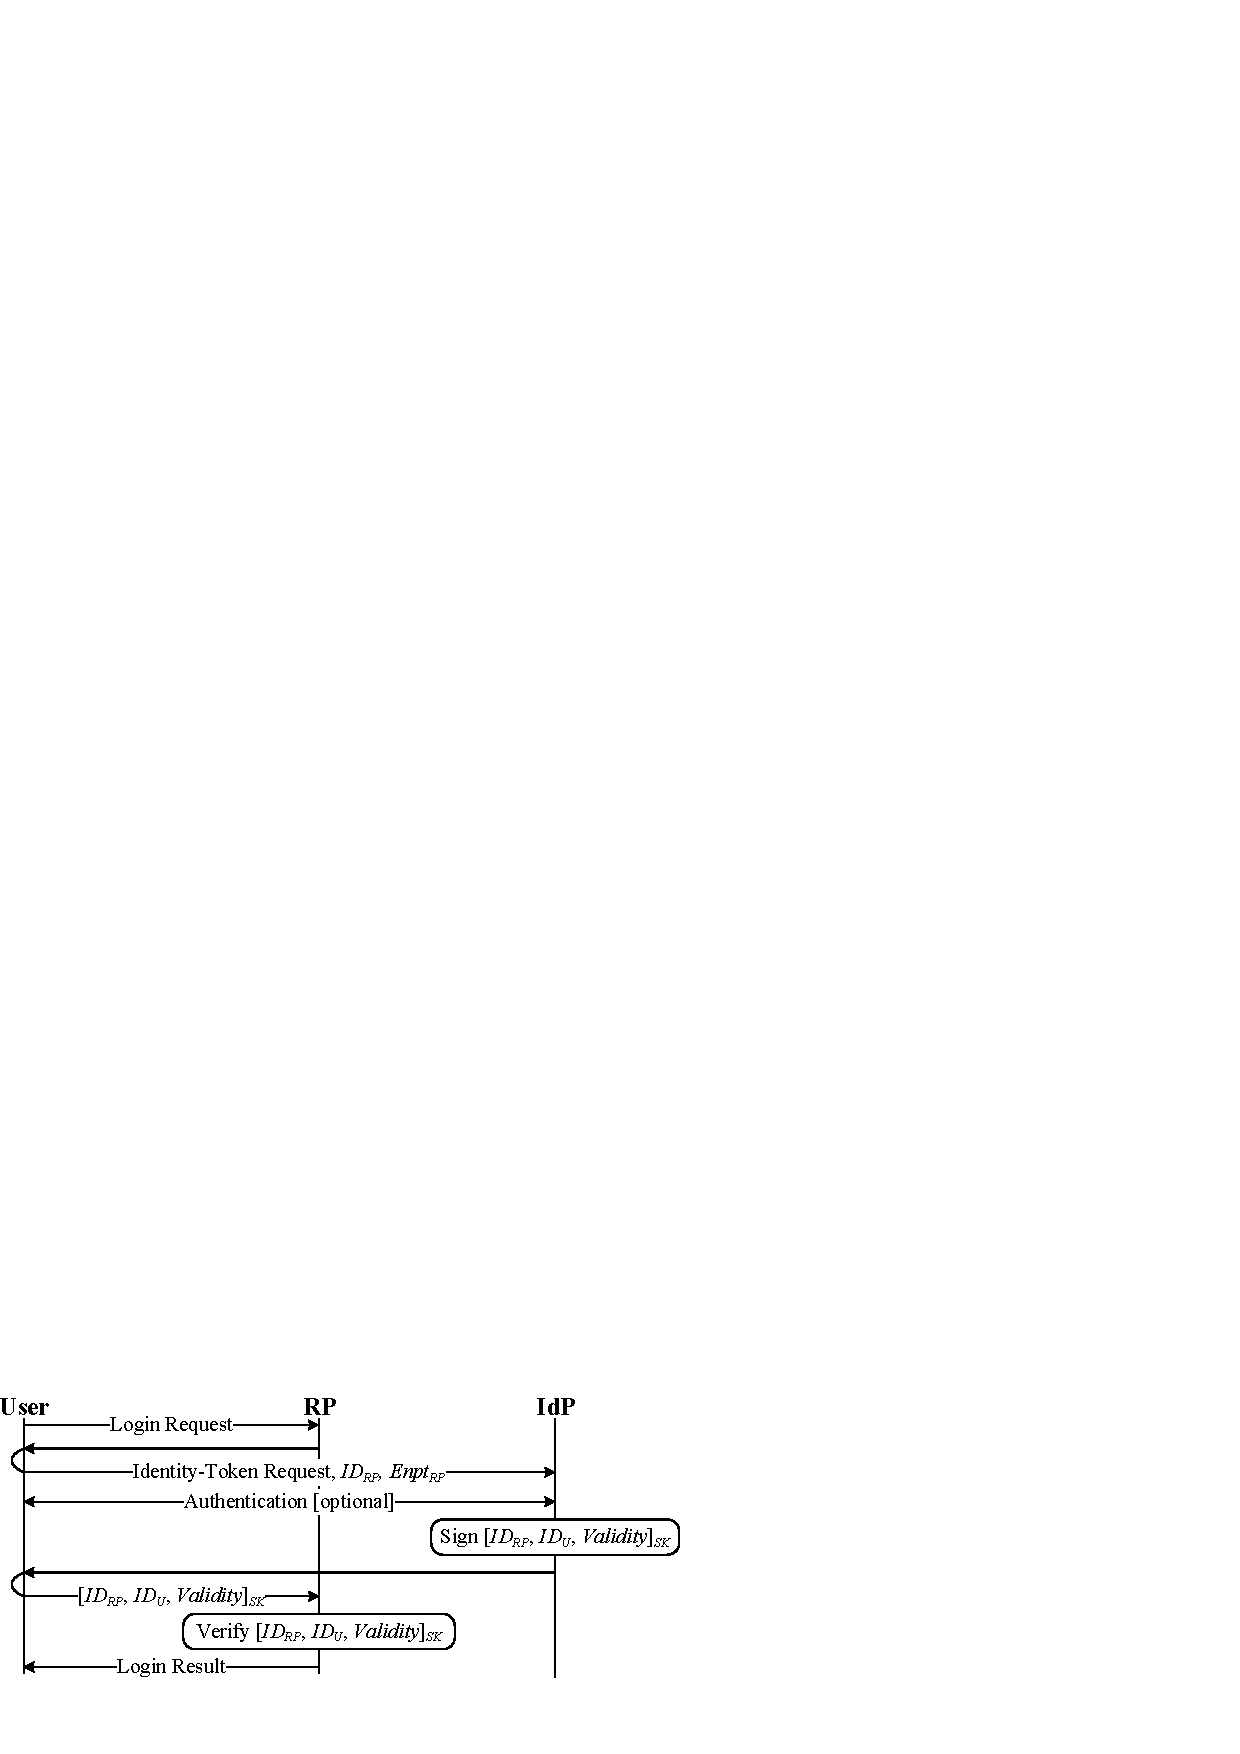
\includegraphics[width=0.95\linewidth]{fig/OIDC.pdf}
  \caption{The implicit SSO login flow of OIDC}
  \label{fig:OpenID}
\end{figure}

\begin{table*}[tb]
\footnotesize
    \caption{Privacy-preserving solutions for SSO and identity federation}
    \centering
    \begin{tabular}{|c|c|c|c|c|c|c|}
  \hline
  \multirow{3}*{\textbf{~~Solution~~}} &
  \multicolumn{3}{c|}{\textbf{SSO Features} - supported $\CIRCLE$, unsupported $\Circle$, or partially $\LEFTcircle$} & \multicolumn{3}{c|}{\textbf{Privacy Threats} - prevented $\CIRCLE$ or not $\Circle$} \\ \cline{2-7}
  & User Identification & User Authentication & IdP-confirmed Selective  & IdP-based & RP-based & Server \\
  & at each RP & only to the IdP &  Attribute Provision & Login Tracing & Identity Linkage & Collusion$^{\dag}$ \\\hline
  OIDC w/ PPID \cite{NIST2017draft} & $\CIRCLE$ & $\CIRCLE$ & $\CIRCLE$ & $\Circle$ & $\CIRCLE$ & $\Circle$ \\ \hline
  BrowserID \cite{BrowserID} & $\CIRCLE$ & $\CIRCLE$$^1$ & $\Circle$ & $\CIRCLE$ & $\Circle$ & $\Circle$ \\ \hline
  SPRESSO \cite{SPRESSO} & $\CIRCLE$ & $\CIRCLE$ & $\LEFTcircle$$^2$ & $\CIRCLE$ & $\Circle$ & $\Circle$ \\ \hline
  MISO \cite{miso} & $\CIRCLE$ & $\CIRCLE$ & $\CIRCLE$ & $\CIRCLE$ & $\CIRCLE$ & $\Circle$$^3$  \\ \hline 
  PRIMA \cite{prima} & $\CIRCLE$ & $\Circle$ & $\CIRCLE$ & $\CIRCLE$ & $\Circle$ & $\Circle$ \\ \hline
  PseudoID \cite{PseudoID} & $\CIRCLE$ & $\Circle$ & $\LEFTcircle$$^4$ & $\CIRCLE$ & $\CIRCLE$ & $\CIRCLE$ \\ \hline
  Opaak \cite{Opaak} & $\LEFTcircle$$^5$ & $\Circle$ & $\Circle$ & $\CIRCLE$ & $\CIRCLE$ & $\CIRCLE$ \\ \hline
  U-Prove \cite{uprov} & $\CIRCLE$ & $\Circle$ & $\LEFTcircle$$^6$ & $\CIRCLE$ & $\CIRCLE$ & $\CIRCLE$ \\ \hline
  UnlimitID \cite{UnlimitID} & $\CIRCLE$ & $\Circle$ & $\CIRCLE$ & $\CIRCLE$ & $\CIRCLE$ & $\CIRCLE$ \\ \hline
  EL PASSO \cite{ELPASSO} & $\CIRCLE$ & $\Circle$ & $\CIRCLE$ & $\CIRCLE$ & $\CIRCLE$ & $\CIRCLE$ \\ \hline
  Fabric Idemix \cite{hyperledge-idemix} & $\LEFTcircle$$^7$ & $\Circle$ & $\CIRCLE$ & $\CIRCLE$ & $\CIRCLE$ & $\CIRCLE$ \\ \hline
 % PrivacyPass \cite{privacypass,trusttoken} & $\Circle$ & $\Circle$ & $\Circle$ & $\CIRCLE$ & $\CIRCLE$ & $\Circle$ \\ \hline
  \usso & $\CIRCLE$ & $\CIRCLE$ & $\CIRCLE$ & $\CIRCLE$ & $\CIRCLE$ & $\Circle$ \\ \hline
\end{tabular}
    \label{tbl:comparison-protocol}
\flushleft
{\footnotesize
$^{\dag}$. This threat happens when all servers involved in the processing of identity tokens collude.\\
1. A BrowserID user generates an \emph{ephemeral} private key to sign subsidiary ``identity assertion'' tokens,
also verified by the RP.\\
2. SPRESSO can be extended to provide selective user attributes in the tokens, while the prototype does not implement this feature.\\
3. MISO is immune to collusive attacks by the IdP and RPs, but another \emph{fully-trusted} server called mixer is involved in the identity-token generation.\\
4. Blindly-signed user attributes can be selectively provided using zero-knowledge proofs but not implemented in the prototype.\\
5. Opaak supports two exclusive pseudonym options: (\emph{a}) linkable within an RP but unlinkable across multiple RPs and (\emph{b}) unlinkable for any pair of actions.\\
6. A U-Prove credential may contain attributes that are \emph{invisible} to the IdP, in addition to the ones confirmed by the IdP. \\
7. In the original design of Idemix \cite{idemix}, every user logs into an RP with a unique account, but Fabric Idemix implements completely-anonymous services.}
\end{table*}

The following three features are desired in SSO services and supported by popular SSO systems \cite{NIST2017draft, OpenIDConnect,rfc6749, SAML, SAMLIdentifier}.

\noindent \textbf{Unique user identification at an RP.}
An RP recognizes each user by a \emph{unique} identity or account at the RP to provide customized services across multiple logins.
Such a non-anonymous SSO system is much more desirable in various scenarios than anonymous services.

\noindent\textbf{User authentication {\em only} to the IdP.}
RPs only verify the identity tokens issued by an IdP, and the authentication between a user and the IdP is typically conducted \emph{independently} of the steps that deal with identity tokens.
This design offers advantages. First, the IdP authenticates users by any appropriate means such as passwords, one-time passwords, or multi-factor authentication.
Meanwhile, a user only maintains her credential at the IdP; and if it is lost or leaked, the user only needs to renew it at the IdP.
However, if a user proves a \emph{non-ephemeral} secret to RPs that is valid across multiple logins, she will have to notify each RP in the events of loss or leakage, or additional revocation checking will be needed \cite{ELPASSO, UnlimitID}.

\noindent\textbf{Selective IdP-confirmed attribute provision.}
An IdP usually includes user attributes in identity tokens \cite{OpenIDConnect,rfc6749} along with user (pseudo-)identities.
A user maintains these attributes at the trusted IdP,
which obtains the user's authorization before enclosing attributes or provides only pre-selected attributes.

\subsection{Privacy-Preserving SSO and Identity Federation}
\label{subsec-solutions}

Privacy-preserving SSO is expected to offer the desired features listed in Section \ref{subsec:OIDC} while addressing different types of privacy threats.
In contrast, privacy-preserving identity federation offers more privacy protections but introduces extra complexity in the user authentication process.
Identity federation enables a user registered at a trusted IdP to be accepted by other parties, potentially with different accounts,
but \emph{additional user operations for the authentication steps between the user and RPs} are involved.\footnote{SSO protocols \cite{OpenIDConnect,rfc6749, SAML, SAMLIdentifier} allow a user to log into an RP \emph{without} maintaining an account at the RP by herself or holding a permanent secret to be verified by the RP. Although the term ``single sign-on (SSO)'' was used in other schemes \cite{PseudoID, Opaak, ELPASSO, WangWS13, HanCSTW18, HanCSTWW20}, they are different from the widely-used SSO protocols because a user needs to maintain the accounts at different RPs and/or hold a permanent secret verified by the RPs. In this paper, we refer to them as \emph{identity federation} to emphasize this difference.}
As shown in Table \ref{tbl:comparison-protocol}, none of the existing solutions 
perfectly satisfies all expectations.


\noindent\textbf{Privacy-preserving SSO.}
Existing privacy-preserving SSO approaches \cite{BrowserID, SPRESSO, NIST2017draft} prevent either IdP-based login tracing or RP-based identity linkage, but not both.
Pairwise pseudonymous identifiers (PPIDs) are specified \cite{OpenIDConnect, SAMLIdentifier} and recommended \cite{NIST2017draft}
for protecting user privacy against curious RPs.
An IdP creates a unique PPID for a user to log into some RP and encloses it in identity tokens, so colluding RPs cannot link the user's identities.
It cannot prevent IdP-based login tracing because the IdP needs the RP's identity to assign PPIDs.

Other privacy-preserving SSO schemes prevent IdP-based login tracing but leave users vulnerable to RP-based identity linkage, due to the unique user identities enclosed in identity tokens.
For example, in BrowserID \cite{BrowserID} %(formerly known as Firefox Accounts \cite{FirefoxAccount} and Mozilla Persona \cite{persona}),
the IdP %(called the primary identity authority in BrowserID)
issues a ``user certificate'' token that binds a user identity to an \emph{ephemeral} public key. The user then signs a subsidiary ``identity assertion'' token that binds the target RP's identity and sends both tokens to the RP. In SPRESSO \cite{SPRESSO} the RP creates a one-time pseudo-identity in each login, which is enclosed in identity tokens along with the user's unique identity.

MISO \cite{miso} decouples the calculation of PPIDs from an IdP,
        and another mixer server calculates a user's PPID
    based on a user identity, the visited RP's identity and a secret key,
    after it receives the authenticated user's identity from the IdP.
MISO prevents both RP-based identity linkag for the RPs receives only PPIDs,
    and IdP-based login tracing because the visited RP is disclosed to the mixer but not the IdP.
It protects a user's online profile against even collusive attacks by the IdP and RPs,
    but it requires an extra fully-trusted mixer server.
  %      which is ensured by Intel SGX.

% 这个就是扯淡吧?为什么还要网络通信呢?直接把Mixer实现在IdP内部,就行了吧?

\noindent\textbf{Privacy-preserving identity federation.}
In PRIMA \cite{prima}, the IdP signs a credential
that binds user attributes and a verification key. Using the signing key, the user selectively provides attributes to the RPs. This verification key works as the user's identity but exposes her to RP-based identity linkage.

To protect user privacy against more threats, PseudoID \cite{PseudoID} introduces a service in addition to the IdP,
 to blindly sign \cite{blind-sign}
an access token that binds a pseudonym and a user secret.
The user then unblinds this token and uses the secret to log into an RP. Approaches based on anonymous credentials \cite{anon-credential-2001, idemix, anon-credential} have been proposed to implement privacy-preserving identity federation \cite{hyperledge-idemix, Opaak, uprov, UnlimitID, ELPASSO}. For instance, the IdP signs anonymous credentials in Opaak \cite{Opaak}, UnlimitID \cite{UnlimitID}, EL PASSO \cite{ELPASSO}, and U-Prove \cite{uprov,uprove-conference}, and binds them with non-ephemeral user secrets. %, with which users can authenticate to an RP.
The users prove ownership of the anonymous credentials using the secrets and disclose IdP-confirmed attributes in the credentials in most approaches except Opaak. Similarly, Hyperledger Fabric \cite{hyperledge-idemix} integrates Idemix anonymous credentials \cite{idemix} for completely-unlinkable pseudonyms and IdP-confirmed attribute disclosure.


These approaches prevent both IdP-based tracing and RP-based identity linkage for (\emph{a}) the RP's identity is not enclosed in the anonymous credentials and (\emph{b}) the user selects different pseudonyms when visiting different RPs.
Furthermore, they protect user privacy against collusive attacks by the IdP and RPs, as \emph{user-managed} pseudonyms cannot be linked through anonymous credentials \cite{anon-credential-2001, idemix, anon-credential} even when the ownership of these credentials is proved to RPs using one secret.
However, this privacy protection results in additional user operations in identity federation, compared with widely-used SSO.
Users are required to maintain not only the authentication credentials for the IdP but also the long-term secrets that are verified by RPs.
For example, EL PASSO \cite{ELPASSO} requires users to keep the secrets securely on their devices and coordinate the credential revocation process \cite{ELPASSO, UnlimitID}.
Besides, the users locally manage their accounts at different RPs. This actually involves authentication steps between the user and RPs, which is usually referred to as \emph{asynchronous authentication} \cite{ELPASSO}.


\noindent\textbf{Anonymous identity federation.}
Such approaches offer strong user privacy protections. They allow users to access RPs with pseudonyms that cannot be used to link any two access actions.
Anonymous identity federation was formalized \cite{WangWS13} and implemented using cryptographic primitives such as group signature and zero-knowledge proof \cite{WangWS13, HanCSTWW20, HanCSTW18}. Special features including proxy re-verification \cite{HanCSTWW20} and designated verification \cite{HanCSTW18}, are also supported. %in these schemes.
%and proposed for different applications such as GSM communications \cite{ElmuftiWRR08},
However, these completely-anonymous authentication services only work for special scenarios and do not support user identification at an RP, which is a common requirement in most applications.

\subsection{Anonymous Tokens and OPRF-based Applications}
\label{sec:related}

PrivacyPass and TrustToken \cite{privacypass,trusttoken} adopted the oblivious pseudo-random function (OPRF) protocol \cite{oprf-proved,voprf-proved,oprf-bitcoin-wallet} to generate anonymous tokens with which authorized users could access resources anonymously.
A user generates a random number $e_i$ to blind an unsigned token $T_i$ into $[e_i]T_i$. After authenticating the user, a token server signs $[e_i]T_i$ with its private key $k$ and returns $[k e_i]T_i$ to the user, who converts it into an anonymous token  ($T_i, [k]T_i$) using $e_i$. In this process, the server obliviously calculates the pseudo-random output (i.e., anonymous token).
The RPs do not identify each user if we use these tokens in an SSO service, because these tokens are completely indistinguishable.

\usso\ applies a similar cryptographic technique in identity transformations  (details in Section \ref{sec:UPPRESSO}).
 A user selects a random number $t_i$ to transform $ID_{RP}$ to $PID_{RP} = [t_i]ID_{RP}$, protecting $ID_{RP}$ from the IdP.
Then, the IdP uses the user's permanent identity $u$ to calculate $PID_U = [u]PID_{RP} = [ut_i]ID_{RP}$,
which is similar to token signing by the token server in PrivacyPass/TrustToken. Hence, \usso\ provides the \emph{IdP-untraceability} property, i.e., the IdP cannot link $ID_{RP}$ and $[t_i]ID_{RP}$, which roughly corresponds to the {\em token signing-redemption unlinkability} in PrivacyPass/TrustToken, i.e., the token server cannot link $T_i$ and $[e_i]T_i$ (or $[k]T_i$ and $[ke_i]T_i$). %($[e_i]T_i, [ke_i]T_i$) and  ($T_i, [k]T_i$).

To support SSO services, \usso\ is required to work among three parties, unlike the two-party OPRF and PrivacyPass/TrustToken protocols.
It leverages this cryptographic technique in different ways for privacy-preserving SSO services. %, unlike the completely anonymous service in PrivacyPass/TrustToken.
%This also requires extending the two-party OPRF protocol to work for three parties in SSO services.
First, \usso\ securely shares the user-selected random number $t_i$ with the target RP,
enabling it to independently derive the user's unique account, i.e., $Acct = [t_i^{-1}]PID_{U}$. This account is ``obliviously'' determined by the IdP when it calculates the user's pseudo-identity based on the ``blinded'' input (i.e., the RP's pseudo-identity). Second, $u$ and $ID_{RP}$, which correspond to $k$ and $T_i$ in PrivacyPass/TrustToken, are designed as the \emph{permanent identities} of the user and the RP, respectively, to establish the relationships between identities obliviously.
This is different from existing OPRF-based systems  \cite{privacypass, trusttoken, strong-oprf, oprf-bitcoin-wallet, pesto, oprf-ot-si, pp-ss, Private-Contact-Discovery, o-kms, oprf-deduplication} that always use $k$ as the server's \emph{secret key}.
The integration of SSO (pseudo-)identities  and OPRF variables requires a deep understanding of both SSO and OPRF protocols.
Finally, \usso\ leverages the OPRF's randomness property to provide \emph{RP unlinkability}, which is not needed in PrivacyPass/TrustToken.
It ensures colluding RPs cannot link any two logins, %i.e., ($ID_{RP}, t, [u]ID_{RP}$) and ($ID_{RP'}, t', [u']ID_{RP'}$),
even by sharing their knowledge about pseudo-identities and permanent accounts related to the logins.
This property offers desirable indistinguishability of \emph{different users} logging into colluding RPs.
It corresponds to the indistinguishability of \emph{different keys} for signing anonymous tokens, not considered in PrivacyPass/TrustToken. % but they intentionally distinguish different keys by configuring a unique public key for each user to verify the signed tokens.

Although \usso\ mathematically employs the same technique in its identity transformations as the OPRF protocol \cite{oprf-proved,voprf-proved}, we prove more properties of these algorithms to ensure security and privacy. % in Theorems 4, 6, and 7.
\usso\ essentially depends on the \emph{obliviousness} property to ensure IdP untraceability, %prevent the IdP from learning any information about $ID_{RP}$ when receiving a token request for $[t_i]ID_{RP}$,
the \emph{deterministicness} property of \emph{pseudo-random} functions to enable the RP to derive a permanent account for any $t$, and the \emph{randomness} property to provide RP unlinkability. %when user identities (i.e., the key secret $k$ of pseudo-random functions) are unknown.
Last but not least, \usso\ requires an additional property for SSO services, called \emph{RP designation}.
It is satisfied \emph{only if} no collision exists in RPs' pseudo-identities (see Lemma \ref{lemma-rp}), which correspond to the blinded inputs of the evaluated pseudo-random function \cite{oprf-proved,voprf-proved}.
This property %, i.e., \emph{collision-freeness of blinded inputs},
is not explicitly required in other OPRF-based solutions and therefore may not be supported by all OPRF protocols. Thus, an OPRF protocol is not always ready to implement identity transformations in \usso, unless no collision exists in the blinded inputs.

\begin{comment}
PrivacyPass and TrustToken \cite{privacypass,trusttoken}
adopted the oblivious pseudo-random function (OPRF) protocol \cite{oprf-proved,voprf-proved,oprf-bitcoin-wallet} to generate anonymous tokens for authorized users to access resources. A user generates a random number $e_i$ for each unsigned token $T_i$ and blinds $T_i$ into $[e_i]T_i$.
Once the user is authenticated, a token server signs $[e_i]T_i$ with a private key $k$ as $[k e_i]T_i$. Then, the user converts $[ke_i]T_i$ to $[k]T_i$ using $e_i$ and redeems the token ($T_i, T_i^k$) to anonymously access resources. \usso\ applies a similar cryptographic skill to design identity transformations. A user transforms $ID_{RP}$ to $PID_{RP} = [t_i]ID_{RP}$ using a random number $t_i$.
Then, the IdP calculates $PID_U = [u]PID_{RP}$ %= [ut]ID_{RP}$
from $PID_{RP}$ using the user's identity $u$. Finally, the visited RP calculates $Acct = [t_i^{-1}]PID_{U}$ from $PID_{U}$ using the shared $t_i$. The \emph{IdP-untraceability} property in \usso, i.e., $[t_i]ID_{RP}$ and $ID_{RP}$ cannot be linked by an IdP, roughly corresponds to the unlinkability between token signing and redemption in PrivacyPass/TrustToken, i.e., ($[e_i]T_i, [ke_i]T_i$) and  ($T_i, [k]T_i$) cannot be linked by the token server.


%%%%%%%%%%%%%%
%%% 以下的段落,我尽量不希望写成“我们直接借鉴OPRF协议来设计”。
%% 原因:1. 的确不是这样;2. 如果我们是直接借鉴OPRF协议来设计UPPRESSO,则后面的行文不应该是现在这样子。我们后面的全文行文,完全是在谈ID transformation的角度。
PrivacyPass/TrustToken adopted the OPRF protocol for token generation, i.e., the server obliviously calculates a pseudo-random output for any user input as tokens, and the anonymous tokens are indistinguishable.
If they are used to realize SSO, the RPs cannot identify each user. In contrast, \usso\ applies this cryptographic skill in different ways from anonymous tokens, to provide a non-anonymous but privacy-preserving SSO service. First, it works for three parties in SSO while OPRFs and PrivacyPass/TrustToken are two-party protocols. In \usso\ a user shares the random number $t$ with an RP, which is used for protecting $ID_{RP}$ and enables the RP to derive the user's account, %at this RP,
and the IdP ``obliviously'' determines the account based on the user identity and the RP's pseudo-identity (or ``blinded'' identity).
In this process, we actually apply pseudo-random functions but uses the \emph{secret key} of pseudo-random functions as a \emph{user identity} (i.e., $u$ in identity transformations), while it is used as \emph{secret keys} in PrivacyPass/TrustToken and other OPRF-based applications \cite{privacypass,trusttoken,strong-oprf,oprf-bitcoin-wallet, pesto,oprf-ot-si,pp-ss, Private-Contact-Discovery,o-kms,oprf-deduplication}.
This unusual application requires a special understanding of the variables in OPRFs and the (pseudo-)identities in SSO services.
%This extension is unlikely to occur in OPFRs that consider $k$ as the private key of the server, but it is reasonable in \usso\ as it uses random numbers as identities and trapdoors to design oblivious pseudo-random functions for identity transformations.
%Compared with the original OPRFs, we use the $k$ key (they are always private keys) as a user identity.

% 第一段:说明2个点:
% 1. 2 party -> 3 party: user把随机数分享给RP。
% 2. 把key用作uid,在SSO中。把prf的输入输出,用作PID和account。
% 他们的token,与uid/account无关
Moreover, \usso\ actually leverages the randomness property of OPRFs to provide \emph{RP unlinkability}, while this property is not needed in PrivacyPass/TrustToken. It ensures colluding RPs cannot link any two logins  across RPs, i.e., ($ID_{RP}, t, [u]ID_{RP}$) and ($ID_{RP'}, t', [u']ID_{RP'}$), even if they share the knowledge about the pseudo-identities and permanent accounts of the users initiating these logins.
In \usso\ this property results in the indistinguishability of \emph{different users} in colluding RPs' view, therefore corresponding to \emph{different keys} for signing anonymous tokens, which is not considered in PrivacyPass/TrustToken. % but they intentionally distinguish different keys by configuring a unique public key for each user to verify the signed tokens.

Although \usso\ employs the same mathematical algorithms in its identity transformations as the OPRF protocol \cite{oprf-proved,voprf-proved}, we prove more properties of these algorithms to ensure security and privacy. % in Theorems 4, 6, and 7.
\usso\ depends on the \emph{obliviousness} property to ensure IdP untraceability, %prevent the IdP from learning any information about $ID_{RP}$ when receiving a token request for $[t_i]ID_{RP}$,
the \emph{deterministicness} property of \emph{pseudo-random} functions to enable the RP to derive a permanent account for any $t$, and the \emph{randomness} property to provide RP unlinkability. %when user identities (i.e., the key secret $k$ of pseudo-random functions) are unknown.
Last but not least, \usso\ requires an additional property for SSO services, called \emph{RP designation}.
It is satisfied \emph{only if} no collision exists in RPs' pseudo-identities (see Lemma 1), which are actually the blinded inputs of the evaluated pseudo-random function \cite{oprf-proved,voprf-proved}.
This property %, i.e., \emph{collision-freeness of blinded inputs},
is not explicitly required in other OPRF-based solutions and therefore may not be supported by all OPRF protocols. Thus, an OPRF protocol is not always ready to implement identity transformations in \usso, unless no collision exists in the blinded inputs.

%For example, we plan to analyze this property of quantum-secure ORPF protocols \cite{ideal-lattice-oprf,isogency-oprf} in the future, to find out whether they work effectively with the identity transformations in \usso.

%\footnote{Due to the extension of three parties and the requirement of input-collisionlessness, we did not realize this cryptographic technique has been published in OPRFs until anonymous reviewers pointed it out.}

\end{comment}

\subsection{Extended Related Work}
%Cryptographic primitives are used for protecting user privacy.
\noindent\textbf{Cryptographic primitives for sign-on privacy.}
Distributed key generation and zero-knowledge proofs are used to generate ring-signature private keys as untraceable pseudonyms \cite{crypto-book} or prove users' statements about their credentials without revealing the credential contents \cite{zklaim}.
One-time key-share tokens \cite{tandem} are generated in two-party threshold cryptography systems to protect users' key-usage patterns.
PESTO \cite{pesto} combines distributed partially-oblivious pseudo-random functions (dpOPRFs) and distributed signatures in proactively-secure SSO services, and signs a commitment of an identity token (but not the token itself) for better user privacy.

%\vspace{0.5mm}
\noindent\textbf{Formal analysis of SSO protocols.}
A formal analysis on SAML-based SSO \cite{ArmandoCCCT08} found that a Google-implemented variant does not bind RP identities correctly in the identity tokens.
Fett et al. \cite{FettKS16, FettKS17} formally analyzed OIDC and OAuth 2.0 using a Dolev-Yao style model \cite{FettKS14} and reported the 307 redirection and IdP mix-up attacks.
In this paper, we also developed a Dolev-Yao style model for \usso, to prove its security and privacy (see Appendix \ref{appendix-model}).



%\vspace{0.5mm}
\noindent\textbf{Implementation vulnerabilities in SSO.}
Various vulnerabilities have been found in several SSO systems for web applications, resulting in attacks %of impersonation and identity injection
that break the confidentiality \cite{WangCW12,ccsSunB12, ArmandoCCCPS13, DiscoveringJCS,dimvaLiM16}, integrity \cite{WangCW12, SomorovskyMSKJ12, WangZLG16, MainkaMS16, MainkaMSW17,dimvaLiM16} or RP designation \cite{WangZLG16, MainkaMS16, MainkaMSW17, YangLCZ18,dimvaLiM16} of identity tokens.
%In the SSO services of Google and Facebook, %from the view of browser-relayed traffics
%    logic flaws of the IdPs and RPs were detected \cite{WangCW12}.  % to break the confidentiality and integrity of identity tokens.
The integrity of identity tokens was violated %\cite{SomorovskyMSKJ12,WangCW12,WangZLG16,MainkaMS16, MainkaMSW17}
due to software flaws such as defective verification by RPs \cite{WangCW12,WangZLG16,MainkaMSW17}, XML signature wrapping \cite{SomorovskyMSKJ12}, and IdP spoofing \cite{MainkaMS16,MainkaMSW17}.
Meanwhile, the RP designation was broken because of incorrect binding by an IdP \cite{YangLCZ18, WangZLG16} or insufficient verification by RPs \cite{MainkaMS16, MainkaMSW17, YangLCZ18}.
A defective IdP does not enclose an identifiable Email address in signed tokens \cite{WangCW12},
 which breaks the user identification.
%Similar vulnerabilities have been found in Android Apps that break the confidentiality \cite{ChenPCTKT14, WangZLLYLG15, YangLS17, ShiWL19}, integrity \cite{ChenPCTKT14, YangLS17}, and RP designation \cite{ChenPCTKT14, ShiWL19, WangZLLYLG15} of SSO identity tokens.

%Navas et al. \cite{NavasB19} discussed the possible attack patterns against OIDC services.
%Automatic tools such as SSOScan \cite{ZhouE14}, OAuthTester \cite{YangLLZH16} and S3KVetter \cite{YangLCZ18},
% detect the violations of confidentiality, integrity, or RP designation of SSO identity tokens.
% Wang et al. \cite{ExplicatingSDK} detect the vulnerable applications
%     built with authentication/authorization SDKs,
%      due to the implicit but unsuitable assumptions of these SDKs.


%Furthermore, if a user is compromised, the attacker can log in to RPs on his behalf. So, we consider malicious users, malicious RPs, and colluding users and RPs in our threat model (see Section \ref{subsec:threatmodel}).





% In a mobile system,
% browsers, IdP Apps,
%     or IdP-provided SDKs %(e.g., an encapsulated WebView)
%          are responsible for forwarding identity tokens, %from the IdP App to RP Apps.
% but none of them ensures an identity token is sent to the designated RP only \cite{ChenPCTKT14, WangZLLYLG15}.
% %    because a WebView or the system browser cannot authenticate the RP Apps and the IdP App may be repackaged.
% %SSO protocols are modified for mobile Apps, but the modifications are not well understood by developers \cite{ChenPCTKT14, YangLS17}.
% Vulnerabilities were found in Android Apps,
%     to break confidentiality \cite{ChenPCTKT14,WangZLLYLG15,YangLS17,ShiWL19}, integrity \cite{ChenPCTKT14,YangLS17}, and RP designation \cite{ChenPCTKT14,ShiWL19} of identity tokens.
% A flaw was found in Google Apps \cite{ArmandoCCCPS13}, allowing a malicious RP to hijack a user's authentication attempt and inject a payload to steal the cookie or identity token belonging to another RP.

% If a user is compromised,
%     attackers will log in to RPs on his behalf.
% Single sign-off helps the victim user
%  to revoke all his tokens accepted and log out from the RPs  \cite{GhasemisharifRC18}.
% FedCM \cite{FedCM} attempts to disable iframe and third-party cookies in SSO, which could be exploited to track users.
% %UPRRSSO protects privacy in SSO through ID transformations and our prototype does NOT use either iframe or third-party cookies.

\section{The Identity-Transformation Approach}
\label{sec:challenge}

We discuss the security requirements of privacy-preserving SSO and present the identity-transformation approach.


\subsection{Security Requirements for SSO Services}
\label{subsec:basicrequirements}

Non-anonymous SSO services \cite{OpenIDConnect,rfc6749,SAML,SAMLIdentifier,NIST2017draft} are designed to allow a \emph{legitimate} user to log into an \emph{honest} RP with her account at this RP, %correlating multiple logins,
by presenting \emph{identity tokens} issued by a \emph{trusted} IdP.
To achieve this goal, the trusted IdP issues an identity token that specifies the RP being accessed (i.e., \emph{RP designation}) and the authenticated user's identity or pseudo-identity (i.e., \emph{user identification}).
An honest RP verifies the RP's identity in the identity token before accepting it and authorizes the token holder to log in as the specified user. This prevents malicious RPs from replaying any received identity tokens to gain unauthorized access to other honest RPs as victim users.
The confidentiality and integrity of identity tokens are also necessary to prevent eavesdropping and tampering. Identity tokens are forwarded to the target RPs by the authenticated user and should not be revealed to any other parties. So they are usually signed by the trusted IdP and transmitted over HTTPS \cite{OpenIDConnect, rfc6749, SAML}.

\begin{figure}[b]
  \centering
  \includegraphics[width=0.99\linewidth]{fig/IDCorrelation.pdf}
  \caption{Identity transformations in \usso} %privacy-preserving SSO}
  \label{fig:IDCorrelation}
\end{figure}

%The requirements for secure SSO services, i.e., RP designation, user identification, integrity, and confidentiality of identity tokens, have been extensively studied \cite{ArmandoCCCT08, SPRESSO, FettKS14, FettKS16, FettKS17}.
%Any vulnerabilities that undermine these properties result in various attacks \cite{SomorovskyMSKJ12, WangCW12, ArmandoCCCPS13, ZhouE14, WangZLLYLG15, WangZLG16, YangLLZH16, MainkaMS16, MainkaMSW17, YangLCZ18, YangLS17, ShiWL19, ChenPCTKT14, ccsSunB12, DiscoveringJCS, dimvaLiM16, CaoSBKVC14, TowardsShehabM14}.

\subsection{Identity Transformation}
\label{subsec:solutions}

We aim to develop a privacy-preserving SSO system that ensures security properties while preventing both IdP-based login tracing and RP-based identity linkage.
In \usso, these requirements are satisfied through \emph{transformed identities} in the identity tokens. Table \ref{tbl:notations-dilemma} lists the notations used in this paper.
The subscript $j$ and/or the superscript $i$ may be ignored if it does not cause ambiguity.

\begin{table}[tb]
\footnotesize
    \caption{The (pseudo-)identities in \usso}
    \centering
%    \begin{tabular}{|l|l|l|}
    \begin{tabular}{|p{1.0cm}|p{5.1cm}|p{1.13cm}|} \hline
    {\textbf{Notation}} & {\textbf{Description}} & {\textbf{Lifecycle}} \\ \hline
    {$ID_U$} & {The user's unique identity at the IdP.} & {Permanent} \\ \hline
    {$ID_{RP_j}$} & {The $j$-th RP's unique identity at the IdP.} & {Permanent} \\ \hline
    {$PID_{U,j}^i$} & {The user's pseudo-identity in her $i$-th login to the $j$-th RP.} & {Ephemeral} \\ \hline
    {$PID_{RP_j}^i$} & {The $j$-th RP's pseudo-identity in the user's $i$-th login to this RP.} & {Ephemeral} \\ \hline
    {$Acct_j$} & {The user's identity (or account) at the $j$-th RP.} & {Permanent} \\ \hline
    \end{tabular}
    \label{tbl:notations-dilemma}
\end{table}

In an SSO login flow, a user initiates the process by negotiating an \emph{ephemeral} pseudo-identity $PID_{RP}$  with the target RP and sending an identity-token request that encloses $PID_{RP}$ to the IdP.
After successfully authenticating the user as $ID_U$, the IdP calculates an \emph{ephemeral} $PID_U$ based on $ID_U$ and $PID_{RP}$ and issues an identity token that binds $PID_U$ and $PID_{RP}$. Upon receiving a token with a matching $PID_{RP}$, the RP calculates the user's \emph{permanent} $Acct$ and authorizes the token holder to log in.
The relationships among the permanent and ephemeral (pseudo-)identities are depicted in Figure \ref{fig:IDCorrelation}, where the \emph{red} and \emph{green} blocks represent \emph{permanent} and \emph{ephemeral} (pseudo-)identities, respectively, and the labeled arrows denote the transformations of (pseudo-)identities.

%An identity token binds the (pseudo-)identities of an authenticated user and an RP.
%Since an IdP authenticates users and then always knows the user's identity (i.e., $ID_U$),
%    to prevent the IdP-based login tracing,
%    we should not reveal the target RP's permanent identity (i.e., $ID_{RP}$) to the IdP.

For RP designation, $PID_{RP}$ should be \emph{uniquely} associated with the target RP.
For user identification, with \emph{ephemeral} $PID_{U}^i$ in each login, the designated RP should be able to derive a unique \emph{permanent} account  (i.e., $Acct$) of the user at this RP.
To prevent IdP-based login tracing, it is essential to ensure that the IdP does not obtain any information about $ID_{RP}$ from any $PID_{RP}^i$.
Thus, in a user's multiple logins to one RP,
 she should generate independent $PID_{RP}^i$s\footnote{The IdP should not be able to link multiple logins visiting a given RP, while the RP's identity is unknown to the IdP.} % the IdP-based login tracing is still effective, to correlate a user's multiple logins.
and independent $PID_U^i$s.\footnote{If $PID_U^i$ is not completely independent of each other, it implies that there is a possibility for the IdP to link multiple logins visiting a given RP.}
Finally, to prevent RP-based identity linkage,
% the IdP does not enclose $ID_U$ in identity tokens.
%a user pseudo-identity (i.e., $PID_U$) is bound instead:
%$PID_U$ is bound in identity tokens:
the RP should not obtain any information about $ID_U$ from any $PID_{U,j}$, which implies that $PID_{U,j}$ for different RPs should also be independent of each other.

We propose three identity transformations as below:
\vspace{-\topsep}\begin{itemize}
\setlength{\topsep}{0pt}
\setlength{\partopsep}{0pt}
\setlength{\itemsep}{0pt}
\setlength{\parsep}{0pt}
\setlength{\parskip}{0pt}
\item
$\mathcal{F}_{PID_{RP}}(ID_{RP}) = PID_{RP}$, calculated by the user and the RP.
In the IdP's view,
$\mathcal{F}_{PID_{RP}}()$ is a one-way function and $PID_{RP}$
is \emph{indistinguishable} from random variables.
\item
$\mathcal{F}_{PID_U}(ID_U, PID_{RP}) = PID_{U}$, calculated by the IdP.
In the target RP's view,
    $\mathcal{F}_{PID_U}()$ is a one-way function and $PID_{U}$ is \emph{indistinguishable} from random variables.
\item
$\mathcal{F}_{Acct}(PID_{U}, PID_{RP}) = Acct$, calculated by the target RP.
Given $ID_U$ and $ID_{RP}$, $Acct$ is %\emph{permanent} and
\emph{unique} to other accounts at this RP.
That is, in a user's two different logins to the RP,
 $\mathcal{F}_{Acct}(PID_{U}^i, PID_{RP}^i) = \mathcal{F}_{Acct}(PID_{U}^{i'}, PID_{RP}^{i'})$.
\end{itemize}




\section{The Designs of \usso}
\label{sec:UPPRESSO}

This section presents the threat model and assumptions, the identity-transformation algorithms, and finally the \usso\ protocol with design specifics for web applications.

\subsection{The Threat Model}
\label{subsec:threatmodel}
The system consists of an honest-but-curious IdP as well as several honest or malicious RPs and users. % or even collude with each other.
This threat model is in line with widely-used SSO services \cite{OpenIDConnect,rfc6749, SAML, SAMLIdentifier}.

%\vspace{0.5mm}
\noindent \textbf{Honest-but-curious IdP.} The IdP strictly follows the protocols,
 while remaining interested in learning about user profiles.
For example, it could store all received messages to infer the relationship between $ID_U$, $ID_{RP}$, $PID_{U}$, and $PID_{RP}$.
 % to track a user's login activities.
It never actively violates the protocols, so a script downloaded from the IdP also strictly follows the protocols (see Section \ref{sec:web-design} for specific designs for web applications).
The IdP maintains the private key well for signing identity tokens and RP certificates, %(see Section \ref{implementations} for details)
which prevents adversaries from forging such messages.

%\vspace{0.5mm}
\noindent \textbf{Malicious users.} Adversaries could control a set of users by stealing their credentials or registering Sybil users in the system.
 Their objective \cite{SPRESSO, FettKS14} is to (\emph{a}) impersonate a victim user at honest RPs or (\emph{b}) entice an honest user to log into an honest RP under another user's account.
A malicious user could modify, insert, drop, or replay messages or even behave arbitrarily in login flows.

\noindent \textbf{Malicious RPs.}
Adversaries could control a set of RPs by registering at the IdP as an RP or exploiting vulnerabilities to compromise some RPs.
Malicious RPs could behave arbitrarily, attempting to compromise the security or privacy guarantees of \usso.
For example, they could manipulate $PID_{RP}$ in a login, attempting to (\emph{a}) entice honest users to return an identity token that could be accepted by some honest RP or (\emph{b}) manipulate the generation of $PID_U$ to analyze the relationship between $ID_U$ and $PID_U$.

%\vspace{0.5mm}
\noindent \textbf{Colluding users and RPs.}
Malicious users and RPs could collude,
 attempting to break the security or privacy guarantees for honest users and RPs.
For example, a malicious RP could collude with malicious users to %steal another user's identity token and
 impersonate a victim at honest RPs or link an honest user's logins visiting colluding RPs.

We do \emph{not} consider the collusion of the IdP and RPs.
If the IdP were to collude with some RPs, a user would complete login flows \emph{entirely} with malicious entities.\footnote{MISO protects user privacy against the collusion of the IdP and RPs, by introducing an extra fully-trusted mixer server.}
In principle, it would require a long-term user secret to protect (or transform) permanent accounts across these RPs.
This secret should be held \emph{only} by the user; otherwise, the colluding IdP and RPs could always link these accounts.
However, the accounts derived from the user secret would need to be updated if the secret was lost or leaked (see more discussions about IdP-RP collusive attacks in Section \ref{sec:discussion}).

Finally, the security and privacy properties of \usso\ are guaranteed against different combinations of the above adversaries.
In particular, it implements secure SSO services against colluding users and RPs,
        while preventing (\emph{a}) IdP-based login tracing by an honest-but-curious IdP
            and (\emph{b}) RP-based identity linkage by colluding RPs and users.

\subsection{Assumptions}
We assume HTTPS is used to secure communications between honest entities, and the cryptographic primitives are secure. The software stack of an honest entity is correctly implemented to transmit messages to receivers as expected.

\usso\ is designed for users who value privacy. We assume a user \emph{never} authorizes the IdP to enclose any \emph{distinctive} attributes, such as telephone number, Email address, etc., in identity tokens or sets such attributes at any RP. Hence, privacy leakages due to re-identification by distinctive attributes across RPs are out of our scope.
In addition, we do not consider the tracking of a user's network activities by network traffic analysis or crafted web pages, as they can be prevented by existing defenses.
For example, FedCM \cite{FedCM} attempts to disable iframe and third-party cookies in SSO, which could be exploited to track users. This work focuses only on the privacy threats introduced by SSO protocols.


%When a user visits multiple RPs concurrently from one browser, a malicious RP may actively redirect his account to another RP server using crafted web pages. Meanwhile, traffic analysis is possible in SSO scenarios, where a user's activities can be tracked from network packets and active account linkage through malicious web pages. We do not consider these attacks in this work, as they can be prevented by existing defenses.


\subsection{Identity-Transformation Algorithms}
\label{subsec:overview}

We design identity-transformation algorithms %  $\mathcal{F}_{PID_{RP}}$, $\mathcal{F}_{PID_{U}}$ and $\mathcal{F}_{Acct}$,
on an elliptic curve $\mathbb{E}$.
Table \ref{tbl:notations-protocol} lists the notations. The subscript $j$ and/or superscript $i$ may be omitted if there is no ambiguity.


\begin{table}[tb]
\footnotesize
    \caption{Notations used in the \usso\ protocol}
    \centering
%    \begin{tabular}{|c|c|c|}
    \begin{tabular}{|p{0.93cm}|p{6.71cm}|} \hline
    {\textbf{Notation}} & {\textbf{Description}} \\ \hline
    {$\mathbb{E}$, $G$, $n$} & {$\mathbb{E}$ is an elliptic curve over a finite field $\mathbb{F}_q$. $G$ is a base point (or generator) on $\mathbb{E}$, and the order of $G$ is a prime number $n$.} \\ \hline
    {$ID_U$} & {$ID_U = u \in [1, n)$ is a user's unique identity at the IdP, which is known only to the IdP.} \\ \hline
   {$ID_{RP_j}$} & {$ID_{RP} = [r]G$ is the $j$-th RP's unique identity, which is publicly known; $r \in [1, n)$ is known to \emph{nobody}.} \\ \hline
    {$t$} & {$t \in [1, n)$ is a user-selected random integer in each login; $t$ is shared with the target RP and kept unknown to the IdP.} \\ \hline
    {$PID_{RP_j}^i$} & {$PID_{RP} = [t]{ID_{RP}} = [tr]G$ is the $j$-th RP's pseudo-identity, in the user's $i$-th login to this RP.} \\ \hline
    {$PID_{U,j}^i$} & {$PID_U = [{ID_U}]{PID_{RP}} = [utr]G$ is the user's pseudo-identity, in the user's $i$-th login to the $j$-th RP.} \\ \hline
     {$Acct_j$} & {$Acct = [t^{-1}\bmod n]PID_{U} = [ID_U]ID_{RP} = [ur]G$ is the user's account at the $j$-th RP.} \\ \hline
    {$SK$, $PK$} & {The IdP's private key and public key, which are used to sign and verify identity tokens and RP certificates.} \\ \hline
%    {$T$} & {The trapdoor to derive $Account$: $T=N_U^{-1} \bmod n$.} \\ \hline
    {$Enpt_{RP_j}$} & {The $j$-th RP's endpoint for receiving the identity tokens.} \\ \hline
    {$Cert_{RP_j}$} & {The IdP-signed RP certificate binding $ID_{RP_j}$ and $Enpt_{RP_j}$.} \\ \hline
%    {$PEnpt_{U,j}^i$} & {A user-generated random "pseudo-endpoint'', in the user's $i$-th login to the $j$-th RP.} \\ \hline
    \end{tabular}
    \label{tbl:notations-protocol}
\end{table}

The IdP assigns a unique random integer $u$ to a user (i.e., $ID_U = u$),
 while randomly selecting $ID_{RP} = [r]G$ for the RP if it is a unique point on $\mathbb{E}$.
Here, $G$ is a point on $\mathbb{E}$ of order $n$, and $[r]G$ denotes the addition of $G$ on the curve $r$ times.


\noindent {\bf $\boldsymbol{ID_{\boldsymbol{RP}}}$-$\boldsymbol{PID_{\boldsymbol{RP}}}$ Transformation.} A user selects a random number $t \in [1, n)$ as the trapdoor and calculates $PID_{RP}$.
\begin{equation}
PID_{RP} = \mathcal{F}_{PID_{RP}}(ID_{RP}) = [t]{ID_{RP}} = [tr]G
\label{equ:PIDRP}
\end{equation}


In each login, the user selects $t$ and shares it with the RP to negotiate $PID_{RP}$. 
%--removed due to double-check discussion
%It makes no difference if the RP selects $t$ randomly and sends it to the user, as long as both of them calculate $PID_{RP}$ \emph{independently} and check if the received $PID_{RP}$ is equal to the calculated one.

\noindent {\bf $\boldsymbol{ID_U}$-$\boldsymbol{PID_U}$ Transformation.}
On receiving an identity-token request for $PID_{RP}$ from a user identified as $ID_U$, the IdP calculates $PID_{U}$ as below.
\begin{equation}
PID_{U} = \mathcal{F}_{PID_U}(ID_U, PID_{RP}) =
  [{ID_U}]{PID_{RP}} = [utr]G
 \label{equ:PIDU}
\end{equation}


\noindent {\bf $\boldsymbol{PID_U}$-$\boldsymbol{Acct}$ Transformation.}
The trapdoor $t$ is sent to the target RP, which checks whether $PID_{RP}$ included in identity tokens equals $[t]ID_{RP}$. After verifying a token that binds $PID_U$ and $PID_{RP}$, it calculates $Acct$ as follows.
\begin{equation}
Acct = \mathcal{F}_{Acct}(PID_{U})
   = [t^{-1} \bmod n]PID_{U}
   \label{equ:Account}
\end{equation}
From Equations \ref{equ:PIDRP}, \ref{equ:PIDU}, and \ref{equ:Account}, it is derived that
\begin{equation}
   Acct =  [t^{-1}utr \bmod n]G = [ur]G = [ID_U]ID_{RP}
   \label{equ:AccountNotChanged}
\end{equation}


With the help of $t$, the RP derives a \emph{unique} account from different identity tokens for the same user in her different logins. It is the user's \emph{permanent} account at this RP. %, which is \emph{unique} among all accounts at the same RP. 
Meanwhile, the user's accounts at different RPs are inherently different and unlinkable (see Section \ref{sec:analysis} for a detailed proof).

%--- remove following the shepherd's comment
% \newc
% In this process, the RP needs to check if $PID_{RP} = [t]ID_{RP}$ holds after extracting $PID_{RP}$ from a received identity token. Otherwise, a malicious user with $ID_{U'} = u'$ could randomly select $t'$ and $u$, and set $PID_{RP}$ as $[t'u'^{-1}][u]ID_{RP}$. Then, the malicious user requests a token from the IdP, in which $PID_{U'} = [ID_{U'}]PID_{RP}=[u'][t'u'^{-1}][u]ID_{RP} = [t'u]ID_{RP}$.
% If the RP does not check the received $PID_{RP}$, it would use the received $PID_{U'}$ to calculate an account as $Acct = [t'^{-1}]PID_{U'}=[u]ID_{RP}$, which is the account of a potential victim user with $ID_{U} = u$.
% The malicious user could repeat the above attacks with random $u \in \mathbb{Z}_n$ until the account of some victim user is calculated by the RP. {\newc If it does not derive an existing account of some honest user, the RP will treat the adversary as a newly-registered user without any alerts.}

% Similarly, if the RP selects $t$ and calculates $PID_{RP}$, the user needs to check whether the received $PID_{RP}$ equals $[t]ID_{RP}$ before requesting an identity token.
% Otherwise, malicious users could impersonate a victim user at some honest RP by colluding with another malicious RP.
% That is, when receiving $PID_{RP}=[t']ID_{RP}$ from the honest RP, the malicious user forwards it to colluding $RP'$, which sends it to the victim user in another login.
% If the victim does not check the received $PID_{RP}$, she would request from the IdP an identity token that binds $PID_U$ and the manipulated $PID_{RP}$ and present the token to the malicious RP.
% This token would allow the malicious user to log into the honest RP under the victim user's account.

\oldc
A user's identity $u$ is kept secret from RPs. Otherwise, colluding RPs could calculate $[u]ID_{RP_j}$s for any known $u$ and link them.
Meanwhile, $ID_{RP} = [r]G$ is publicly-known but $r$ is unknown to RPs.
%The IdP never discloses $r$ to RPs.
Otherwise, two colluding RPs with $ID_{RP_j} = [r]G$ and $ID_{RP_{j'}} = [r']G$ could link a user's accounts by checking whether $[r']Acct_j = [r]Acct_{j'}$ holds.
%enumerate the user's accounts by calculating  and link them.


\subsection{The Design Specifics for Web Applications}
\label{sec:web-design}

In commonly-used SSO protocols \cite{OpenIDConnect,rfc6749, SAML, SAMLIdentifier},
an IdP needs to know the visited RP to ensure the confidentiality of identity tokens. For instance, in OIDC services, an RP's endpoint to receive tokens is stored as the \verb+redirect_uri+ parameter at the IdP.
The IdP employs HTTP 302 redirection to send identity tokens to the RP, by setting this parameter as the target URL in the HTTP responses to a user's identity-token request \cite{OpenIDConnect}, so the user agent forwards it to the designated RP.
However, in \usso, the IdP does not know about the visited RPs, requiring a user agent by itself to calculate $PID_{RP}$ and send identity tokens to the RP's endpoint.
%In UPPRESSO, the IdP is not aware of visited RPs, so user agents (or browsers) are responsible for forwarding the identity token to the intended RP and computing $PID_{RP}$. On the contrary, in commonly-used SSO protocols \cite{OpenIDConnect,rfc6749,SAML,SAMLIdentifier}, the IdP requires this information to ensure the \emph{confidentiality} of identity tokens. For instance, in OIDC services, an RP's endpoint URL is set as the \verb+redirect_uri+ parameter \cite{OpenIDConnect} during registration to receive tokens. When transmitting identity tokens to an RP, the IdP employs HTTP 302 redirection. This endpoint is the target URL in HTTP responses, allowing the browser to forward it to the designated RP.

\usso\ supports commercial-off-the-shelf (COTS) browsers to work as the user agent and implements the user-agent functions using web scripts in browsers. The scripts are responsible for communications with the origin web servers,
 and downloaded from the IdP and the visited RP, respectively. It is worth noting that a script downloaded from an honest entity is considered \emph{honest}.

The IdP script is necessary because the RP script could leak its origin to the IdP web server due to the automatic inclusion of an HTTP \verb+referer+ header in all HTTP requests it sends.
Besides, the IdP script is trusted to interact with the users for attribute authorization,
 %and ensure the confidentiality of identity tokens, i.e., a token is sent to only the designated RP,
%% 机密性这一句没有必要写,因为“如果RP是malicious,则RP总是可以将token泄露出去”。
  while the RP (and its script) could be malicious.
Thus, on receiving an identity-token request, the IdP web server checks the \verb+referer+ header to ensure it is sent by the IdP script.

The RP script is responsible for preparing $ID_{RP}$ and $Enpt_{RP}$ for the IdP script, through an RP certificate issued by the IdP. %It binds the RP's identity and endpoint. %(i.e., $ID_{RP}$ and $Enpt_{RP}$).
In each login, the RP script sends the certificate to the IdP script, which then verifies it and extracts $ID_{RP}$ and $Enpt_{RP}$.
The same as in widely-adopted SSO systems \cite{OpenIDConnect, rfc6749, SAML, SAMLIdentifier}, in \usso\ a user does not need to configure anything locally as the IdP's public key is already set in the IdP script.

After receiving an identity token from the IdP, the IdP script needs to ensure the RP script will forward the token to $Enpt_{RP}$ %, which is bound with $ID_{RP}$
specified in the RP certificate.
As the communication between the scripts occurs within the COTS browser using the \verb+postMessage+ HTML5 API, %To avoid the honest user sending the identity token to an adversary,
we use the \verb+postMessage+ targetOrigin mechanism \cite{postm-targeto} to restrict the recipient. %(i.e., the RP script).
 When the IdP script sends messages, the recipient's origin is set as a parameter, such as \verb+postMessage(tk, 'https://RP.com')+, which includes the protocol (e.g., \verb+https+), the domain (e.g., \verb+RP.com+), and a port if applicable.
Only the script downloaded from this targetOrigin is considered a legitimate recipient.

%The \emph{RP certificates} deals with the problem of mapping an identity proof with its targeting RP.
%That is, the IdP script derives the RP's $ID_{RP}$ and origin from the RP certificate, while the $PID_{RP}$ is generated with this $ID_{RP}$. Thus, the IdP script always knows the targeting RP of identity proof, therefore, the \verb+postMessage+ mechanism can guarantee that the identity proof would not be sent to the adversary.

As discussed in Section \ref{subsec:overview}, a user needs to calculate $PID_{RP} = [t]ID_{RP}$ based on $ID_{RP}$ extracted from the RP certificate. Thus, this function should be implemented by an \emph{honest} script that does not leak $t$ to the IdP, from which it could calculate $ID_{RP} = [t^{-1}\bmod n]PID_{RP}$. In \usso, we consider the IdP script honest; otherwise, it could directly leak the RP's domain to the IdP.
To mitigate this risk, we can implement the user agent with trusted browser extensions, which need to be installed by users before visiting RPs.

\begin{figure*}[htb]
  \centering
  \includegraphics[height=0.55\textheight]{fig/process-js.pdf}
  \caption{The SSO login flow of \usso}
  \label{fig:process}
\end{figure*}

When a user is visiting an RP, the browser downloads the RP script, which in turn opens a new window to download the IdP script. To prevent referer leakage during the download of the IdP script, we need to ensure the HTTP request does not automatically carry a \verb+referer+ header, which reveals the visited RP's domain to the IdP. %Generally, when a browser window visits another website not belonging to its opener's origin, the HTTP request to this website automatically carries a \verb+referer+ header (i.e., the opener's origin). Such an HTTP header leaks the visited RP's domain to the IdP.
In \usso, this new window is a \emph{redirection} from the RP to the IdP (Steps 1.2-1.3 in Figure \ref{fig:process}), but not a direct visit by the browser.
The HTTP response from the RP includes a \verb+referrer-policy=no-referrer+ header, which ensures that the HTTP request to download the IdP script carries no \verb+referer+ header.
This approach is specified by W3C \cite{referer_policy} and widely supported. We have tested it in various browsers such as Chrome, Safari, Edge, Opera, and Firefox, and confirmed that no referer leakage occurs.




\subsection{The \usso\ protocol}
\label{implementations}

\noindent \textbf{System Initialization.}
An IdP generates a key pair ($SK$, $PK$) to sign and verify identity tokens and RP certificates.
%The IdP keeps $SK$ secret, and $PK$ is publicly known.

\vspace{1.5mm}
\noindent\textbf{RP Registration.}
%Each RP launches an initial registration operation to finish configurations.
Each RP registers itself at the IdP to obtain $ID_{RP}$ and its RP certificate $Cert_{RP}$ as follows:
\vspace{-\topsep}\begin{enumerate}
\setlength{\topsep}{0pt}
\setlength{\partopsep}{0pt}
\setlength{\itemsep}{0pt}
\setlength{\parsep}{0pt}
\setlength{\parskip}{0pt}
\item
An RP pre-installs $PK$ by trusted means.
It sends a registration request, including the endpoint to receive identity tokens and other information.
\item
The IdP randomly selects a \emph{unique} point on $\mathbb{E}$,
        and assigns it to $ID_{RP}$.
Thus, $ID_{RP} = [r]G$ but $r$ is known to \emph{nobody} due to the elliptic curve discrete logarithm problem (ECDLP).
%random number $r \in [1,n)$ until $ID_{RP} = [r]G$ is unique.
 %   but $r$ is kept unknown to the RP.
It then signs $Cert_{RP} = [ID_{RP}, Enpt_{RP}, *]_{SK}$,
     where $[\cdot]_{SK}$ is a message signed using $SK$ and $*$ is supplementary information such as the RP's common name.
\item
The RP verifies $Cert_{RP}$ using $PK$, and accepts $ID_{RP}$ and $Cert_{RP}$ if they are valid.
\end{enumerate}


%\vspace{0.5mm}
\noindent\textbf{User Registration.}
Each user registers once at the IdP. She sets up her unique username and the corresponding credential.
The IdP will then assign
a unique random identity $ID_U = u \in [1, n)$ to the user.
$ID_U$ is known only to the IdP internally.
%This is similar to the steps in existing SSO systems.


\vspace{1.5mm}
\noindent\textbf{SSO Login.} A login %is typically launched through a browser,
%when a user attempts to visit an RP. It
involves four steps: script downloading, RP identity transformation, identity-token generation, and $Acct$ calculation. In Figure \ref{fig:process}, the IdP's and RP's operations are connected by two vertical lines, respectively. The user operations are split into two groups in different browser windows by two vertical lines, one communicating with the IdP and the other with the RP. Solid horizontal lines indicate messages exchanged between the user and the IdP (or the RP), while dotted lines represent a \verb+postMessage+ invocation between two scripts (or browser windows) within the browser.


\vspace{0.85mm}
\noindent 1. {\em Script Downloading.}
The browser downloads scripts from the visited RP and the IdP.
\vspace{-\topsep}
\begin{itemize}
\setlength{\topsep}{0pt}
\setlength{\partopsep}{0pt}
\setlength{\itemsep}{0pt}
\setlength{\parsep}{0pt}
\setlength{\parskip}{0pt}
\item[1.1]
When requesting any protected resources at the RP, the user downloads the RP script.
\item[1.2]
The RP script opens a window in the browser to visit the login path at the RP, which is then redirected to the IdP.
\item[1.3]
The redirection to the IdP downloads the IdP script.
\end{itemize}



%\vspace{1mm}
\noindent 2. {\em RP Identity Transformation.}
The user and the RP negotiate $PID_{RP} = [t]{ID_{RP}}$.
\vspace{-\topsep}
\begin{itemize}
\setlength{\topsep}{0pt}
\setlength{\partopsep}{0pt}
\setlength{\itemsep}{0pt}
\setlength{\parsep}{0pt}
\setlength{\parskip}{0pt}
\item[2.1] The IdP script chooses a random number $t \in [1, n)$ and sends it to the RP script through \verb+postMessage+. The RP script then forwards $t$ to the RP.
\item[2.2] The RP verifies if the received $t$ is an integer in $[1, n)$ and
%Upon receiving $t$, the RP verifies $1 \leq t < n$ and %calculates $PID_{RP}$.
%To acknowledge the negotiation of $PID_{RP}$, The RP
replies with $Cert_{RP}$ and the scope of the requested user attributes. The reply is then transmitted through the RP script to the IdP script.  % through \verb+postMessage+.
\item[2.3] The IdP script verifies $Cert_{RP}$, extracts $ID_{RP}$ and $Enpt_{RP}$ from $Cert_{RP}$, and calculates $PID_{RP}=[t]{ID_{RP}}$.
%It then creates a random endpoint $PEnpt_{U}$ for this login,
 %   to receive identity tokens from the IdP.
    % as the RP endpoint required by IdP.我们已经修改了协议, IdP并不require什么

\end{itemize}


%\vspace{1mm}
\noindent 3. {\em Identity-Token Generation.}
The IdP calculates $PID_U = [ID_U]{PID_{RP}}$ and signs an identity token. % The processes are as follows.
\vspace{-\topsep}
\begin{itemize}
\setlength{\topsep}{0pt}
\setlength{\partopsep}{0pt}
\setlength{\itemsep}{0pt}
\setlength{\parsep}{0pt}
\setlength{\parskip}{0pt}
\item[3.1]
The IdP script sends an identity-token request for $PID_{RP}$ on behalf of the user. %and the user attributes.
 %by checking whether this user is authenticated by IdP.

\item[3.2] The IdP authenticates the user, if not authenticated yet.

\item [3.3]
The IdP script obtains the user's authorization for the requested attributes locally and then sends the scope of the authorized attributes.
Then, the IdP checks if the received $PID_{RP}$ is a point on $\mathbb{E}$,
calculates $PID_U = [ID_U]{PID_{RP}}$, and signs $[PID_{RP}, PID_U, Issuer, Validity, Attr]_{SK}$, where $Issuer$ is the IdP, $Validity$ indicates the validity period, and $Attr$ contains the authorized user attributes.
\item[3.4] The IdP replies with the identity token to the IdP script.
\end{itemize}

%\vspace{1mm}
\noindent 4. {\em $Acct$ Calculation.}
The RP receives the identity token and authorizes the user to log in.
\vspace{-\topsep}
\begin{itemize}
\setlength{\topsep}{0pt}
\setlength{\partopsep}{0pt}
\setlength{\itemsep}{0pt}
\setlength{\parsep}{0pt}
\setlength{\parskip}{0pt}
\item [4.1]
The IdP script forwards the identity token to the RP script,
    which then sends it to the RP through $Enpt_{RP}$.
\item[4.2] The RP verifies the digital signature and the validity period of the token 
%\newc
%Then, the RP extracts $PID_{RP}$ from the token, checks if it equals $[t]ID_{RP}$,
%\oldc
and calculates $Acct = [t^{-1}]{PID_U}$.

\item [4.3] The RP authorizes the user to log in as $Acct$.

\end{itemize}


If any verification fails, this flow will be terminated immediately.
For example, the user halts it when receiving an invalid $Cert_{RP}$.
The IdP rejects an identity-token request in Step 3.3 if the received $PID_{RP}$ is not a point on $\mathbb{E}$, and the RP rejects a token in Step 4.2 if the digital signature is invalid. 
%%%%%%%%%%%%%%%%%%%%%%%%%%%%%%%%%%%%%%%%%%%%%%%%%%%%%%%%%%
% u泄露,则RP有必要比较!否则,就会伤害security。
%or the enclosed $PID_{RP}$ is not equal to $[t]ID_{RP}$.
%%%%%%%%%%%%%%%%%%%%%%%%%%%%%%%%%%%%%%%%%%%%%%%%%%%%%%%%%%
% 分析结论是:
% 现有的简化协议(RP不比较$PID_{RP}$是否相等),则:
% 当u不泄露,u的security和privacy都没有问题;
% 当u泄露,u的security和privacy都没有问题。
%
% 改进协议(RP比较$PID_{RP}$是否相等),则:
% 当u不泄露,u的security和privacy都没有问题;
% 当u泄露,u的security没有问题,u的privacy有问题。
%%%%%%%%%%%%%%%%%%%%%%%%%%%%%%%%%%%%%%%%%%%%%%%%%%%%%%%%%%

\subsection{Compatibility with OIDC}
\label{subsec:compatible}

Both \usso\ and OIDC work with COTS browsers. %Among the four steps of the login flow
In \usso, the \emph{script downloading} step prepares the user agent, which assists the communications with the IdP and RP servers. \usso\ employs web scripts to hide the RP's endpoint from the IdP, while securely forwarding identity tokens to the RP through $Enpt_{RP}$ extracted from the signed RP certificate.
% that protects the identity token from being sent to adversaries. 这句话与Compatibility无关
Therefore, the IdP does not set \verb+redirect_uri+ in the HTTP responses, which is different from OIDC where HTTP redirections are used to implement these communications. Most operations in the \emph{RP identity transformation} step take place within browsers. The RP only receives $t$ to generate an RP pseudo-identity and responds with $Cert_{RP}$,
%The calculation of $PID_{RP}$ is viewed as the operation to prepare an RP identity in OIDC,
which is viewed as a supplementary message to users.
%The operations in the $PID_{RP}$ registration are almost identical to those in the RP Dynamic Registration of OIDC \cite{DynamicRegistration}, except that in OIDC the IdP assigns the RP's identity  while in UPPRESSO this (pseudo-)identity is generated by the registered entity. Besides, the $PID_{RP}$ registration has a validity period.
Consequently, compared to the original OIDC protocol, \usso\ simplifies the IdP's operations in these two steps, while allowing RPs to customize their ``dynamic'' pseudo-identities.

The operations of \emph{identity-token generation} and \emph{$Acct$ calculation} in \usso\ are \emph{identical} to those in OIDC,
 because (\emph{a}) the calculation of $PID_U$ in \usso\ can be viewed as a method to generate PPIDs in OIDC and (\emph{b}) the calculation of $Acct$ can be viewed as a mapping from the user identity in tokens to an account at the RP.

The compatibility is experimentally confirmed through our prototype implementation, which modifies only 23 lines of Java code in MITREid Connect \cite{MITREid}, an open-source OIDC system, to build an IdP of \usso\ (see Section \ref{subsec:proto-imple}).
%It will help the adoption and deployment of UPPRESSO.


\section{Security and Privacy Analysis}
\label{sec:analysis}

%We define three adversarial scenarios under the threat model in Section \ref{subsec:threatmodel}, develop a Dolev-Yao style model \cite{BrowserID} to formalize the SSO login flow in \usso, and then integrate its conclusions to formally prove the security and privacy guarantees provided by \usso.

We formally prove the security and privacy guarantees provided by \usso.
It is worth noting that these guarantees are proved against different adversaries.

% \newc
% \subsection{Adversarial Scenarios}

% Based on our design goals (i.e., the desired security and privacy guarantees) and the potential adversaries discussed in Section \ref{subsec:threatmodel}, we consider three adversarial scenarios as below.

% \noindent\textbf{Adversaries against security.} Malicious users could collude with each other and even with malicious RPs, attempting to (\emph{a}) impersonate an honest user to log into an honest RP or (\emph{b}) entice an honest user to log into an honest RP under a malicious user's account.

% \noindent\textbf{Adversaries against IdP untraceability.}
% The honest-but-curious IdP tries to infer the identities of the RPs that a user requests to access. %or link multiple logins to any RP initiated by a user.

% \noindent\textbf{Adversaries against RP unlinkability.}
% Malicious RPs could collude with each other and even with malicious users, attempting to link logins across these RPs that are initiated by honest users. 
%\oldc


% \subsection{The Dolev-Yao Style Model for \usso}
% \label{dy-model}

% We develop a Dolev-Yao style model \cite{BrowserID, SPRESSO, FettKS16, FettKS17} for \usso, referred to as the \emph{\dyu\ model}, to formalize the login flow of \usso.
% % Dolev-Yao style models abstract cryptographic concepts into an algebra of symbolic messages to discover structural flaws using simple formal logic. % which has been used in the formal analysis of SSO protocols such as OAuth 2.0 \cite{FettKS16} and OIDC \cite{FettKS17}.
% The model abstracts the entities in a web system, such as web servers and browsers, as atomic processes, %which communicate with each other through events. % such as HTTPS requests and responses.
% and defines scripting processes to formulate client-side scripts.
% %The script is dependently invoked by the browser to process the server-defined logic.%such as verifying $Certificate_{RP}$. %postmessage events; %atomic process <-> scripting process, communication. %Other events change self-trigger.
% The atomic processes of \usso\ include an IdP process, a finite set of web servers for honest RPs, a finite set of honest browsers, and a finite set of attacker processes that model malicious RPs and malicious users.
% A browser may invoke an honest IdP script and multiple RP scripts that could be honest or malicious.
% The processes communicate with each other through events such as HTTPS requests and responses,
% %Although the scripts coexist in the same browser, they are strictly separated.
% except that the scripting processes communicate with each other through \verb+postMessage+ which are modeled as transmitted-to-itself events of a browser process.
% %To clearly indicate the action of postMessage communication, we define it as the transmitting-to-itself event of the browser (which is not defined in SPRESSO).

% \newc
% Applying the \dyu\ model, we trace the lifecycle of an identity token from its generation at the IdP to its acceptance at an RP, locate the places where $PID_U$, $PID_{RP}$, and other elements related to the identity token such as $t$ and $u$ are processed, and locate the places where $PK$ is transmitted and used in the IdP script.
% We confirm the following conclusions in the \dyu\ model:
% (\emph{a}) an identity token binding pseudo-identities of honest entities, cannot be leaked to any malicious process;
% (\emph{b}) pseudo-identities and other elements in verified identity tokens cannot be manipulated by any malicious process;
% (\emph{c}) the IdP's public key set in the IdP script cannot be replaced or tampered with by any malicious process, within an honest browser;
% (\emph{d}) the IdP receives nothing about $t$ shared between two honest processes;
% (\emph{e}) $r$ is not leaked to any malicious process as it never leaves the IdP;
% and (\emph{f}) the RPs cannot receive anything about $u$ shared between two honest processes.


\subsection{Security}
\label{analysis-security}

Based on the threat model in Section \ref{subsec:threatmodel}, the adversary against security w.r.t. authentication \cite{FettKS14,BrowserID,SPRESSO} compromises some users, colluding with malicious RPs, and attempts to (\emph{a}) impersonate an honest user to log into an honest RP (i.e., \emph{impersonation}), or (\emph{b}) break the login of an honest user to an honest RP so that the honest user is authenticated as another user (i.e., \emph{identity injection}). 

%could collude with each other and even with malicious RPs, attempting to (\emph{a}) impersonate an honest user to log into an honest RP or (\emph{b}) entice an honest user to log into an honest RP under a malicious user's account.

\newc
For the analysis of security w.r.t. authentication, we develop a formal model of \usso\ web systems (denoted as $\mathcal{U\!W\!S}^{Auth}$), which is defined in Appendix \ref{appendix-model}. It contains an IdP, a finite set of RPs, a finite set of users (i.e., browsers), and a network attacker. The attacker subsumes all web attackers and is assumed to be able to  corrupt a set of users and RPs.


%------- new Theorem 5, move to the beginning of the proof ---------
\begin{thm}
\textsc{(Security)} \emph{\usso\ provides a secure SSO service w.r.t. authentication}.
\label{thm-security}
\end{thm}

\noindent\textbf{\textsc{Proof.}} Every SSO system should satisfy two fundamental properties that are deduced from \cite{FettKS14} and summarized in \cite{BrowserID,SPRESSO}: {\bf (A)} the attacker should not be able to access services of an honest RP as an honest user, and {\bf (B)} the attacker should not be able to authenticate an honest user to an honest RP on behalf of another user, which are formally defined in Definitions 2 and 3 in Appendix \ref{appendix-security}. For the proofs, we demonstrate that both properties are fulfilled for every $\mathcal{UWS}^{Auth}$. 

Before proving Properties {\bf A} and {\bf B}, we first show that a network attacker cannot obtain any information from or manipulate the identity token request from a user (browser) to the IdP, referred to as Property {\bf C1}. Meanwhile, a network attacker cannot obtain any information from or alter the identity token from the IdP to the target RP through the user (browser), referred to as Property {\bf C2}. We adopted the general web system properties shown in the full version of \cite{FettKS14} and followed the approaches in \cite{BrowserID,SPRESSO}, which are based on a Dolev-Yao-style model, and prove them with Lemmas 2-6 in Appendix~\ref{appendix-security}. 

To prove Property {\bf A}, we show that the attacker cannot obtain any useful information from any login of an honest user to an honest RP, which would allow him to impersonate an honest user at some honest RP. In particular, he cannot know the identity-token request (and its $PID_{RP}$) according to Property {\bf C1} nor a valid identity token of the honest user if they are not initiated by a corrupted user or intended for a corrupted RP, according to Property {\bf C1}.  

Meanwhile, we prove that Property {\bf A} is still fulfilled in the following two adversarial scenarios. First, consider a malicious user initiating a login to an honest RP. He selects a random $t$ to share with this RP and then manipulates $PID_{RP}$ to be $[t']ID_{RP}$ instead of $[t]ID_{RP}$ when requesting for an identity token. We prove in Theorem \ref{thm-user-id} that, by showing the identity token with a manipulated $PID_{RP}$ to this honest RP, the malicious user cannot be recognized under the account of any existing honest user at this RP (i.e., {\em User Identification}). Secondly, we consider a malicious $RP$ sharing with a malicious user $U$ the identity token $TK$ that it received from an honest user $U'$. With $TK$, if the malicious $RP$ is able to find $t'$ satisfying $[t']ID_{RP'}=[t]ID_{RP}$ for any honest $RP'$, it could share $TK$ and $t'$ with the malicious user, enabling him to log into $RP'$ on behalf of $U$. We prove in Lemma \ref{lemma-rp} and Theorem \ref{thm-rp-designation} that a malicious RP receiving $t$ and $[t]ID_{RP}$ for $U$'s login cannot find such $t'$, since $PID_{RP}$ in $TK$ is uniquely associated with $t$ and the login to the designated RP (i.e., {\em RP Designation}).

%a network attacker cannot alter: (1) communications between an honest user and an honest RP through restricted \verb+postMessage+ messages between the honest IdP script and RP script (within the user's browser) and obtain or manipulate the secret element $t$;  

To prove property {\bf B}, we first prove in Theorem \ref{thm-user-id}: when an honest user logs into an honest RP, the identity token $TK$ that binds $PID_U$ and $PID_{RP}$ uniquely identifies a user account for this user at the designated RP (i.e., {\em User Identification}). Therefore, an honest user would not be authenticated by an honest RP as any other users in the system.

Meanwhile, we show that the attacker cannot manipulate any login of an honest user to an honest RP in a way that the honest user is mistakenly authenticated as another user. 
%In particular, we show a property of $\mathcal{UWS}^{Auth}$, i.e., a network attacker cannot tamper with $ID_{RP}$ extracted from the RP's certificate. 
In particular, we show that the network attacker cannot tamper with identity token requesting (i.e., Property \textbf{C1} and Lemma 7 in Appendix~\ref{appendix-security}), and therefore he cannot manipulate $ID_{RP}$, which is extracted from the RP's certificate, and $PID_{RP}$, which is computed as $PID_{RP}=[t]ID_{RP}$, to trigger a token for another user while returning it to the victim user. Besides, the attacker cannot manipulate the returned identity token directly based on Property \textbf{C2}. 
%Then, we show that the attacker cannot manipulate $PID_{RP}$ in the identity token request of the honest user (i.e., Property \textbf{C1}), nor the identity token $TK$ issued by the IdP to the honest user and the target honest RP (i.e., Property \textbf{C2}); that is,
%\emph{Token Integrity} is ensured. 
\hfill $\square$

%------- old Theorem 5 ---------
\begin{comment}
\begin{thm}
\textsc{(Security)} \emph{\usso\ provides secure authentication services.}
\end{thm}

\noindent\textbf{\textsc{Proof.}}
According to the formal analysis on SSO security \cite{SPRESSO, FettKS14},
    an SSO system satisfying the following two requirements provides \emph{secure} authentication services in the first adversarial scenario: (\emph{a}) an adversary never obtains a valid identity token issued for an honest user and presents it to an honest RP, and (\emph{b}) an honest user never presents a valid identity token that is not issued for herself to an honest RP.

Following the login flow of \usso, because the integrity and confidentiality of identity tokens are satisfied in Theorems \ref{thm-integrity} and \ref{thm-confidentiality},
 no adversary could obtain a valid identity token that is issued to an honest user for accessing an honest RP. %and accepted by an honest RP.
Meanwhile, if an adversary presents an identity token to an honest RP, which may be issued to the adversary for accessing another RP or to an honest user for accessing a colluding RP, RP designation and user identification, proved in Theorems \ref{thm-rp-designation} and \ref{thm-user-id}, ensure that the honest RP does not derive an honest user's account from this identity token.
%Meanwhile, $PID_U$ can only be calculated by the IdP and the user, since no one else knows or could intercept $u$ according to the DYU model. \oldc

According to the login flow and the \dyu\ model, an honest user always obtains identity tokens issued to herself, because $PID_U$ is calculated based on her identity. 
%% which is protected against adversaries. 这一句,对于security没有用,protecting u是用于privacy。
The confidentiality and integrity of identity tokens ensure that an honest user never presents any token issued for someone else to an honest RP. Finally, with user identification,\footnote{\newc RP designation is a precondition of user identification in \usso, but this is not always necessary for other SSO systems.} her identity tokens are always associated with her account at the target RP.
%According to the conclusions of the DYU model, $PID_U$ is calculated based on the user when the IdP issues an identity token for an authenticated user.
%Moreover, because the confidentiality and integrity of identity tokens are satisfied, an honest user never presents a valid token that is issued to other users.
%When the user identification is satisfied, this token always derives this honest user's account.
%So, an honest user never presents an identity token that is accepted by an honest RP to derive another user’s account at this RP.

Thus, \usso\ is a secure SSO system.
\hfill $\square$

%Finally, according to Theorems 1, 2, 3, 4, and 5, UPPRESSO is secure.

\end{comment}


%We prove that identity tokens in \usso\ and the enclosed pseudo-identities satisfy four properties, namely, \emph{RP designation}, \emph{user identification}, \emph{token confidentiality}, and \emph{token integrity}, which together ensure the security of \usso\ in the first adversarial scenario.

\vspace{2mm}
Next, we prove that \usso\ provides the ``RP Designation'' and ``User Identification'' properties that are used in Theorem \ref{thm-security}. Let us consider an identity token $TK$ binding $PID_{RP}$ and $PID_U$, which is generated by the IdP upon a request from an authenticated user with $ID_U$.

\begin{thm}
\textsc{(RP Designation of $TK$)}  \emph{$PID_{RP}$ in $TK$ uniquely designates an RP with $ID_{RP}$ and receiving $t$ in \usso, where $PID_{RP}= [t]ID_{RP}$, $t \in [1,n)$, $ID_{RP} = [r]G$, $r$ is a random number known only to the IdP, and $G$ is a generator on $\mathbb{E}$ of order $n$.}
\label{thm-rp-designation}
\end{thm}

\noindent\textbf{\textsc{Proof.}} In \usso, $PID_{RP}=[t]ID_{RP}$ is generated by a user based on the target RP's identity $ID_{RP}$ and a user-selected random number $t \in [1,n)$.
%The target RP with $ID_{RP}$ receives $t$, and it will also calculate $PID_{RP}=[t]ID_{RP}$ to match $PID_{RP}$ extracted from a token received.
%It is computationally easy for any party who knows $ID_{RP}$ and $t$ to validate the $PID_{RP}$ in an identity token. A valid
Thus, $PID_{RP}$ always specifies an RP, i.e., %$PID_{RP}$ sent by a user in her identity-token request is calculated as $PID_{RP} = [t]ID_{RP}$, where $ID_{RP}$ is the target RP's identity and $t$ is a random number selected by the user and shared with this RP.
designates the target RP that knows $t$. 
Moreover, according to Lemma \ref{lemma-rp}, given $PID_{RP} = [t]ID_{RP}$, the probability that $PID_{RP}$ designates another RP with $ID_{RP'}$ is \emph{negligible}. %This means that $PID_{RP}$ cannot be associated with any other RPs in the system.
Therefore, $PID_{RP}$ designates only the target RP with $ID_{RP}$ in the system.  \hfill $\square$


\begin{lemma}
\emph{Given any two RPs in a finite set of RPs in \usso,
 the probability that an adversary finds different numbers $t$ and $t' \in [1,n)$ satisfying $[t]ID_{RP_j} = [t']ID_{RP_{j'}}$ is negligible, where $ID_{RP_j}=[r]G$, $ID_{RP_{j'}}=[r']G$, $r$ and $r'$ are different numbers unknown to the adversary, and $G$ is a generator on $\mathbb{E}$ of order $n$.}
\label{lemma-rp}
\end{lemma}


\oldc
\noindent\textbf{\textsc{Proof.}}
Finding $t$ and $t'$ that satisfy $[t]ID_{RP_j} = [t']ID_{RP_{j'}}$, can be described as a $PID_{RP}$-collision game $\mathcal{G}_c$ between an adversary and a challenger: the adversary receives from the challenger a finite set of RP identities, i.e., $ID_{RP_1}$, ..., $ID_{RP_m}$, where $m$ is the number of RPs in the system, and outputs $(a, b, t, t')$ where $a \neq b$. If $[t]ID_{RP_a}=[t']ID_{RP_b}$, which occurs with a probability ${\rm Pr}_s$, the adversary succeeds in this game.
%The attack success probability is defined as ${\rm Pr}_s$.

As depicted in Figure \ref{fig:ecdlp_algorithm}, we design a probabilistic polynomial time (PPT) algorithm $\mathcal{D}^*_c$ based on $\mathcal{G}_c$, to solve the ECDLP: find a number $x \in \mathbb{Z}_n$ satisfying $Q = [x]G$, where $Q$ is a point on $\mathbb{E}$ and $G$ is a generator on $\mathbb{E}$ of order $n$.

%where ${\rm Pr}\{\}$ denotes the probability.
%where $k$ denotes the security parameter and $\epsilon_{c}(k)$ becomes negligible when $k$ is sufficiently large.
%For any sufficiently large $k$, $m \ll 2^k$ since $m$ is a finite integer.

\begin{figure}[tb]
  \centering
  \includegraphics[width=0.96\linewidth]{fig/ecdlp_algorithm.pdf}
  \caption{The PPT algorithm $\mathcal{D}^*_c$ constructed based on the $PID_{RP}$ collision game to solve the ECDLP.}
  \label{fig:ecdlp_algorithm}
\end{figure}

The algorithm $\mathcal{D}^*_c$ works as below.
The input of $\mathcal{D}^*_c$ is in the form of ($G, Q$). On receiving an input ($G$, $Q$), the challenger first randomly chooses $r_1, \cdots, r_m$ in $\mathbb{Z}_n$ to calculate $[r_1]G, \cdots, [r_m]G$.
Then, it randomly chooses $j \in [1,m]$, replaces $[r_j]G$ with $Q$, and sends $m$ RP identities to the adversary, which returns the result ($a$, $b$, $t$, $t'$). Finally, the challenger calculates $s = t^{-1}t'r_b \bmod n$ and returns $s$ as the output of $\mathcal{D}^*_c$.

If the adversary succeeds in $\mathcal{G}_c$ and $[r_a]G$ happens to be replaced with $Q$, then $\mathcal{D}^*_c$ outputs $s=t^{-1}t'r_b =x$ because $[tr_a]G = [t]Q = [t'r_b]G$. For the adversary, $Q$ is indistinguishable from any other RP identities in the input set, as $[r_j]G$ is randomly replaced by the challenger.
Hence, the probability of solving the ECDLP using $\mathcal{D}^*_c$ is formulated as:
\begin{equation*}
{\rm Pr}\{\mathcal{D}^*_c(G, [x]G)=x\} = {\rm Pr}\{s = x\}={\rm Pr}\{a=j\}{\rm Pr}_s=\frac{1}{m}{\rm Pr}_s
\end{equation*}

If the probability of finding $t$ and $t'$ satisfying $[t]ID_{RP_j} = [t']ID_{RP_{j'}}$ is non-negligible, the adversary would have advantages  in $\mathcal{G}_c$ and ${\rm Pr}_s$ is non-negligible regardless of the security parameter $\lambda$.
Thus, we would find that ${\rm Pr}\{\mathcal{D}^*_c(G, [x]G)=x\}$ also becomes non-negligible even when $\lambda$ is sufficiently large, because $m$ is a finite integer and $m \ll 2^\lambda$.
\oldc
This violates the ECDLP assumption. Therefore, the probability of finding $t$ and $t'$ that satisfy $[t]ID_{RP_j} = [t']ID_{RP_{j'}}$ is negligible. \hfill $\square$

\newc
\begin{thm}
\textsc{(User Identification of $TK$)} \emph{$PID_U= [ID_U]PID_{RP}$ in $TK$ uniquely identifies an account at the RP designated by $PID_{RP}$ if and only if it receives $t$ where $PID_{RP} = [t]ID_{RP}$ holds, and this account is uniquely mapped to a user with $ID_U$.}
\label{thm-user-id}
\end{thm}

\noindent\textbf{\textsc{Proof.}}
To issue an identity token requested for $PID_{RP}$, the honest IdP authenticates the user with $ID_U$ and calculates $PID_U = [ID_U]PID_{RP}$, following Equation \ref{equ:PIDU}. The RP designated by $PID_{RP}$ should have received a $t$ from the user. Following Equation \ref{equ:AccountNotChanged}, it can calculate $Acct = [t^{-1}]PID_{U} = [ID_U]ID_{RP}$, which is a \emph{permanent} identifier determined by $ID_U$ and $ID_{RP}$ after the user and the RP register at the IdP. $ID_{RP} = [r]G$ is a generator on $\mathbb{E}$ of order $n$, as $\mathbb{E}$ is a finite cyclic group. Therefore, given a user with $ID_U$, $Acct$ is a \emph{unique} point on $\mathbb{E}$ for any $u \in [1, n)$, and it is \emph{uniquely} associated with $ID_U=u$. 
%We first prove that $PID_{U}$ \emph{uniquely} identifies one account at the designated RP and one user in the system. 
This proves that $PID_U$ in $TK$ identifies an account $Acct$ at the designated RP, which is uniquely mapped to a user with $ID_U$ in the system.

Next, we consider two adversarial scenarios where the attacker replays a token $TK$ for another user to (1) the designated RP but receiving $t'\neq t$ in this login, and (2) any other honest RP with $ID_{RP'} = [r']G \neq [r]G$ (i.e., $r' \neq r$). In the first case, the designated RP would calculate an account as $[t'^{-1}]PID_U = [t'^{-1}ut]ID_{RP}$.
Because a user's identity is randomly selected by the IdP in $\mathbb{Z}_n$ and known only to the user (and the honest IdP), the probability that $t'^{-1}ut$ happens to be the identity of another user is negligible, when $n$ is sufficiently large. As a result, $[t'^{-1}]PID_U$ is likely not to identify any known account at the RP and therefore would be treated as a new account by the RP. 
Secondly, the attacker presents $TK$ to $RP'$ in the system, where $ID_{RP'} = [r']G \neq [r]G$. $RP'$ would calculate the account as $Acct' = [\tilde{t}^{-1}]PID_{U} = [\tilde{t}^{-1}utrr'^{-1}][r']G = [\tilde{t}^{-1}utrr'^{-1}]ID_{RP'}$. The probability that $\tilde{t}^{-1}utrr'^{-1}$ happens to be the identity of another user at $RP'$ is also negligible, when $n$ is sufficiently large. 
%it identifies no account mapped to a user, at any RP not designated by $PID_{RP}$.
\hfill $\square$


%---- remove Theorem 4 and 5 and move the proofs to Appendix
% \newc
% \begin{thm}
% \textsc{(Token Integrity)} \emph{An identity token issued by the IdP cannot be forged or manipulated.}
% \label{thm-integrity}
% \end{thm}

% \noindent\textbf{\textsc{Proof.}} Identity tokens are generated and signed by the honest IdP using its private key, which is sufficiently protected at the IdP against adversaries.
% %Meanwhile, the IdP's public key $PK$ is sent from the IdP to the RPs.
% %and $PK$ which are pre-installed by an RP cannot be manipulated by adversaries.
% With the pre-installed public key, an RP verifies the identity tokens it receives and rejects any forged or manipulated identity tokens. Finally, according to the conclusions of the DYU model, the elements in a verified token cannot be manipulated by malicious entities.
% \hfill $\square$


% \begin{thm}
% \textsc{(Token Confidentiality)} \emph{An identity token is accessible only to its designated RP, besides the requesting user and the IdP.}
% \label{thm-confidentiality}
% \end{thm}

% \noindent\textbf{\textsc{Proof.}}
% An identity token is generated by the IdP and then sent to the requesting user (i.e., its IdP script).
% The IdP script verifies if $ID_{RP}$ specified in a verified RP certificate is designated by $PID_{RP}$ in the identity token and forwards the token to the correct RP script, which is downloaded from the origin of $Enpt_{RP}$ specified also in the RP certificate. %Because the IdP script calculates $PID_{RP} =[t]ID_{RP}$ based on $ID_{RP}$ in this verified RP certificate, this RP is designated in the identity token and will receive the token from the RP script.
% As all the communications between the IdP, RPs, and users are protected by HTTPS and two scripts communicate with each other through restricted \verb+postMessage+ HTML5 channels, according to the conclusions of the \dyu\ model, the identity tokens cannot be leaked to any other entities. \hfill $\square$

%--- End of Theorem 4 and 5
\oldc

\subsection{Privacy against IdP-based Login Tracing}
\label{subsec:IdP-privacy}

As depicted in Section \ref{subsec:threatmodel}, the IdP would attempt to infer the RP's identity visited by a user. Since the IdP is considered \emph{honest-but-curious}, it only collects information from the login requests to infer the visited RPs' identities but does not tamper with the authentication process or deviate from the SSO protocol.
The curious IdP does not collude with others.

\newc
To show \usso\ preventing such \emph{IdP-based login tracing}, we first prove that in $\mathcal{UWS}^{Auth}$, the IdP cannot obtain any information related to the target RP in each login (e.g., $ID_{RP}$, $t$, RP's $EndPoint$) except its \emph{ephemeral} pseudo-identity $PID_{RP}$ (with Property {\bf C1}). Then, we prove in Theorem \ref{thm-idp-untraceability} that with these $PID_{RP}$s in the identity token requests from the users, the IdP cannot (\emph{a}) associate multiple logins to the same RP, or (\emph{b}) distinguish a login to one RP from other logins to another RP, because $PID_{RP}$ is \emph{indistinguishable} from any random variables to the IdP. So, \usso\ prevents \emph{an honest-but-curious IdP} from tracing a user's login activities.

\begin{lemma}
\textsc{(IdP Untraceability)} \emph{In \usso, the IdP cannot distinguish $PID_{RP} = [t]ID_{RP}$ from a random variable on $\mathbb{E}$, where $t$ is random in $\mathbb{Z}_n$.}
\label{lemma-idp-untraceability}
\end{lemma}

\noindent\textbf{\textsc{Proof.}}
Consider a finite cyclic group $\mathbb{E}$ where the number of points on $\mathbb{E}$ is $n$.
Because $G$ is a generator of order $n$, $ID_{RP} = [r]G$ is also a generator on $\mathbb{E}$ of order $n$. %According to the formal model in Appendix \ref{appendix-model}, 
$t$ is randomly chosen in $\mathbb{Z}_n$ and always kept unknown to the IdP. Therefore, $PID_{RP} = [t]ID_{RP}$ is \emph{indistinguishable} from a point $Q$ that is randomly chosen on $\mathbb{E}$ \cite{oprf-proved,voprf-proved}.\footnote{\newc This property has been actually proved in OPRFs \cite{oprf-proved,voprf-proved}, where the OPRF server works similarly to the IdP and learns \emph{nothing} about a client's inputs or outputs of the evaluated pseudo-random function.} \hfill $\square$

\oldc

\subsection{Privacy against RP-based Identity Linkage}
\label{subsec:RP-privacy}

As depicted in the threat model, malicious RPs,
which could collude with some malicious users,
aim to infer the identities of honest users
    or link an honest user's accounts across these RPs.
They attempt to (1) steal the user's identity $ID_U$ directly,
% (2) steal information from or tamper with pseudo-identity transformations in login sessions,
 or (2) link the pseudo-identities of an honest user that are used in her logins to multiple malicious RPs. 


\newc
In each login, an RP obtains \emph{only} a random number $t$ and an identity token enclosing $PID_{RP}$ and $PID_U$. From the token, it learns only an ephemeral pseudo-identifier $PID_{U} = [{ID_U}]{PID_{RP}}$ of the user, from which it deduces a permanent pseudo-identifier $Acct = [ID_U]ID_{RP}$. However, it cannot derive $ID_U$ from $PID_{U}$ or $Acct$ as it is an ECDLP hard problem.

Next, we show that, with Property {\bf C1}, \usso\ prevents malicious RP(s) from reading or altering the identity token request sent by the IdP script that runs in an honest browser to the IdP. Therefore, the RP obtains no knowledge about the user identity $ID_U$. Meanwhile, following the formal model in Appendix \ref{appendix-model}, we see that the RP script running in an honest browser is always honest, no matter if the RP would be corrupted at a later time or not. A script download from a malicious RP would not be installed by an honest user. 

Finally, we prove in Theorem 5 that even if malicious RPs collude with each other and malicious users by sharing $PID_U$s and other information observed in all the logins, they still cannot link any login from an honest user to any other logins from any other honest users to malicious RPs.

%\usso\ prevents the privacy threats of \emph{RP-based identity linkage} against \emph{malicious RPs which collude with malicious users}, attempting to link the logins initiated by an honest user but visiting different colluding RPs. 
%The IdP does not collude with the adversaries in this scenario.

%Therefore, the colluding adversaries share all logins visiting malicious RPs, and attempt to leverage the logins initiated by malicious users to link the other logins by honest users.


With the trapdoor $t$, $PID_{RP}$ and $PID_U$ can be easily transformed into $ID_{RP}$ and $Acct$, respectively, and vice versa. Therefore, we denote the information that an RP learns from a login as a tuple $L$, where $L =(ID_{RP}, t, Acct)=(ID_{RP}, t, [ID_{U}]ID_{RP})=([r]G, t, [ur]G)$.


%Hence, an $RP_j$ with $w$ logins knows $\{L_{1,j},...,L_{w,j}\}$.

When $c$ malicious RPs collude with each other, they create a shared view of all their logins, denoted as $\mathbb{L}$.
%some of which are initiated by honest users and denoted as $\mathbb{L}^h$, and the others by $v$ malicious users  are $\mathbb{L}^m = \mathbb{L} \setminus \mathbb{L}^h$.
When they collude further with $v$ malicious users, the logins initiated by these malicious users are picked out and linked together as
$\mathfrak{L}^m=\left \{ \begin{matrix}
L^m_{1,1},&L^m_{1,2},&\cdots,&L^m_{1,c}\\
L^m_{2,1},& L^m_{2,2},&\cdots,&L^m_{2,c}\\
\cdots,&\cdots,&L^m_{i,j},&\cdots\\
L^m_{v,1},&L^m_{v,2},&\cdots,&L^m_{v,c}
\end{matrix}\right\}$,
where $L^m_{i, j}=([r_j]G, t_{i,j}, [u_ir_j]G)$ for $1 \le i \le v$ and $1 \le j \le c$, and $L^m_{i,j} \in \mathbb{L}$. Any login in $\mathbb{L}$ but not linked in $\mathfrak{L}^m$ is initiated by an honest user to one of the $c$ malicious RPs.


\begin{thm}
\textsc{(RP Unlinkability)} \emph{In \usso, given $\mathbb{L}$ and $\mathfrak{L}^m$, $c$ malicious RPs and $v$ malicious users cannot link any login from an honest user to a malicious RP to any subset of logins from honest users to any other malicious RPs.}
\end{thm}


\noindent\textbf{\textsc{Proof.}} From the logins in $\mathbb{L}$,
 we randomly choose one login $L' \neq L^m_{i,j}$,
 which is from an (unknown) honest user with $ID_{U'}=u'$ to a malicious $RP_a$ and $a \in [1,c]$.
Then, we randomly choose another malicious $RP_b$, where $b \in [1,c]$ and $b \neq a$.
Consider any subset $\mathbb{L}''$ of $w$ logins visiting $RP_b$ by unknown honest users,
 we denote the identities of the honest users who initiate these logins as $\mathbf{u}_w=\{{u''_1}, {u''_2}, \cdots, {u''_w}\}$.
Next, we prove that the colluding adversaries cannot decide if $u'$ is in $\mathbf{u}_w$ or randomly selected from the universal user set.
This indicates the colluding adversaries cannot link $L'$ to another login visiting $RP_b$
    or to another subset of logins visiting $RP_b$.

We first define an RP-based linkage game $\mathcal{G}_r$ between an adversary and a challenger, which describes this login linkage privacy threat: the adversary receives $\mathfrak{L}^m$, $L'$, and $\mathbb{L}''$ from the challenger and outputs $s$, where $s = 1$ if it decides $u'$ is in $\mathbf{u}_w$ %$\{{U''_1}, {U''_2}, \cdots, {U''_w}\}$
and $s=0$ if it believes $u'$ is randomly chosen from the universal user set.
Thus, the adversary succeeds in $\mathcal{G}_r$ with an advantage $\mathbf{Adv}$:
\begin{align*}
%&{\rm Pr}_1={\rm Pr}\{\mathcal{G}_r(\mathfrak{L}, L', \mathbb{L}'' | u' \in \{{u''_1}, {u''_2}, \cdots, {u''_w}\})=1\} \\
&{\rm Pr}_1={\rm Pr}(\mathcal{G}_r(\mathfrak{L}^m, L', \mathbb{L}'')=1 \;| \; u' \in \mathbf{u}_w)  \\
%&{\rm Pr}_2={\rm Pr}\{\mathcal{G}_r(\mathfrak{L}, L', \mathbb{L}'' | u' \in \mathbb{Z}_n)=1\}\\
&{\rm Pr}_2={\rm Pr}(\mathcal{G}_r(\mathfrak{L}^m, L', \mathbb{L}'')=1 \; | \; u' \in \mathbb{Z}_n)\\
&{\mathbf{Adv}}=|{\rm Pr}_1-{\rm Pr}_2|
\end{align*}

As depicted in Figure \ref{fig:dalgorithm}, we design a PPT algorithm $\mathcal{D}^*_r$ based on $\mathcal{G}_r$ to solve the elliptic curve decisional Diffie-Hellman (ECDDH) problem: given $(G, [x]G$, $[y]G$, $[z]G)$, decide whether $z$ is equal to $xy$ or randomly chosen in $\mathbb{Z}_n$, where $G$ is a point on an elliptic curve $\mathbb{E}$ of order $n$, and $x$ and $y$ are integers randomly and independently chosen in $\mathbb{Z}_n$.


\begin{figure}[tb]
  \centering
  \includegraphics[width=1.0\linewidth]{fig/rp-linkage-game.pdf}
  \caption{\newc The PPT algorithm $\mathcal{D}^*_r$ constructed based on the RP-based linkage game to solve the ECDDH problem.}
  \label{fig:dalgorithm}
\end{figure}


The algorithm $\mathcal{D}^*_r$ works as below. (1) Upon receiving an input $(G, Q_1=[x]G, Q_2=[y]G, Q_3=[z]G)$, %of $\mathcal{D}^*_r$
the challenger
chooses random numbers in $\mathbb{Z}_n$ to construct $\{u_i\}$, $\{r_j\}$, and $\{t_{i, j}\}$ for $1 \le i \le v$ and $1 \le j \le c$, with which it assembles $L^m_{i, j}=([r_j]G, t_{i,j}, [u_ir_j]G)$.
In this process, it ensures $[r_{j}]G \neq Q_2$ so that $r_j \neq y$.  % 这个应该反过来讲;因为y是离散对数。
(2) It randomly chooses $a \in [1, c]$ and $t' \in \mathbb{Z}_n$, to assemble $L' = ([r_{a}]G, t', [r_{a}]Q_1) = ([r_{a}]G, t', [xr_{a}]G)$.
(3)
% Here, $L'$ represents the knowledge of the login visiting $RP_{j'}$ by a user with $ID_U = x$.
Next, the challenger randomly chooses $b \in [1, c]$ and $b \neq a$, and replaces $ID_{RP_b}$ with $Q_2 = [y]G$.
Hence, for $1 \le i \le v$, the challenger replaces $L^m_{i, b}=([r_b]G, t_{i,b}, [u_ir_b]G)$ with $(Q_2, t_{i,b}, [u_i]Q_2) = ([y]G, t_{i,b}, [u_iy]G)$, and then constructs $\mathfrak{L}^m$.
(4) the challenger chooses random numbers in $\mathbb{Z}_n$ to construct $\{u''_k\}$ and $\{t''_k\}$ for $1 \leq k \leq w$,
 with which it assembles $\mathbb{L}'' = \{L''_{k; 1\leq k \leq w}\} = \{(Q_2, t''_k, [u''_k]Q_2)\} = \{([y]G, t''_k, [u''_ky]G)\}$.
In this process, it ensures that $[u''_k]G \neq Q_1$ (i.e., $u''_k \neq x$) and $u''_k \neq u_i$,
 for $1 \le i \le v$ and $1 \le k \le w$.
Finally, it randomly chooses $d \in [1, w]$ and replaces $L''_{d}$ with $(Q_2, t''_d, Q_3) = ([y]G, t''_d, [z]G)$.
 Thus, $\mathbb{L}'' = \{L''_{k;1\leq k \leq w}\}$ represents the logins initiated by $w$ honest users, i.e., $\mathbf{u}_w=\{u''_1, u''_2, \cdots, u''_{d-1}, z/y, u''_{d+1}, \cdots, u''_w\}$.
 (5) When the adversary of $\mathcal{G}_r$ receives $\mathfrak{L}^m$, $L'$, and $\mathbb{L}''$ from the challenger, it returns $s$ as the output of $\mathcal{D}^*_r$.

According to the above construction, % of $\mathfrak{L}$, $L'$ and $\mathbb{L}''$,
$x$ is embedded as $ID_{U'}$ in the login $L'$ visiting the RP with $ID_{RP_{a}} = [r_{a}]G$,
and $z/y$ is embedded as $ID_{U''_d}$ in $\mathbb{L}''$ visiting the RP with $ID_{RP_{b}}=[y]G$,
together with $\{u''_1, \cdots, u''_{d-1}, u''_{d+1}, \cdots, u''_w\}$.
Meanwhile, $[r_{a}]G$ and $[y]G$ are two malicious RPs' identities in $\mathfrak{L}^m$.
Because $x \neq u''_{k; 1\leq k \leq w, k \neq d}$ and then $x$ is not in $\{u''_1, \cdots, u''_{d-1}, u''_{d+1}, \cdots, u''_w\}$, the adversary outputs $s=1$ and succeeds in the game \emph{only if} $x = z/y$.
% 这里不是if and only if. "if, 就变成了the adversary必胜了;并不是,而是“有显著的概率”"
% 当“the adversary outputs s=1 且 succeeds in the game”,=> "x = z/y"
% 但是,"x = z/y"  => 不能推导得到“the adversary outputs s=1 且 succeeds in the game”。因为adversary有时候fail、不总是succeed
 Therefore, using $\mathcal{D}^*_r$ to solve the ECDDH problem, we have an advantage $\mathbf{Adv}^*=|{\rm Pr}^*_1 - {\rm Pr}^*_2|$, where
\begin{align*}
&{\rm Pr}^*_1 =  {\rm Pr}(\mathcal{D}^*_r(G, [x]G, [y]G, [xy]G)=1) \\
=&{\rm Pr}(\mathcal{G}_r(\mathfrak{L}^m, L', \mathbb{L}'')=1 \; | \; u' \in \mathbf{u}_w) = {\rm Pr}_1 \\
&{\rm Pr}^*_2= {\rm Pr}(\mathcal{D}^*_r(G, [x]G, [y]G, [z]G)=1) \\
=&{\rm Pr}(\mathcal{G}_r(\mathfrak{L}^m, L', \mathbb{L}'')=1 \; | \; u' \in \mathbb{Z}_n) = {\rm Pr}_2 \\
&\mathbf{Adv}^*=|{\rm Pr}^*_1-{\rm Pr}^*_2|=|{\rm Pr}_1-{\rm Pr}_2|={\mathbf{Adv}}
\end{align*}

If in $\mathcal{G}_r$ the adversary has a non-negligible advantage, then $\mathbf{Adv}^*={\mathbf{Adv}}$ is also non-negligible regardless of the security parameter $\lambda$. This violates the ECDDH assumption. Therefore, the adversary has no advantage in $\mathcal{G}_r$ and cannot decide whether $L'$ is initiated by some user with an identity in $\mathbf{u}_w$ or by a user in the universal user set.
Moreover, because $RP_b$ is any malicious RP, this proof can be easily extended from $RP_b$ to more colluding malicious RPs.
\hfill $\square$

\oldc



%\input{chap_Compact/uid.tex}

\section{Implementation and Evaluation}
\label{sec:implementation}

We implemented a prototype of \usso\footnote{The prototype is open-sourced at https://github.com/uppresso/.} and conducted experimental comparisons with two open-source SSO systems: (\emph{a}) MITREid Connect \cite{MITREid}, which is a PPID-enhanced OIDC system to prevent RP-based identity linkage, and (\emph{b}) SPRESSO \cite{SPRESSO}, which prevents IdP-based login tracing.


\subsection{Prototype Implementation}
\label{subsec:proto-imple}

The \usso\ prototype implemented identity transformations on the NIST P256 elliptic curve, with RSA-2048 and SHA-256 serving as the digital signature and hash algorithms, respectively. The IdP and RP scripts consist of approximately 160 and 140 lines of JavaScript code, respectively.  %to provide the functions in Steps 2.1, 2.3, and 4.3.
The cryptographic computations such as $Cert_{RP}$ verification and $PID_{RP}$ negotiation are performed using jsrsasign \cite{jsrsasign}, an open-source JavaScript cryptographic library.

The IdP was developed on MITREid Connect\cite{MITREid}, a Java implementation of OIDC, %certificated by the OpenID Foundation \cite{OIDF},
with minimal code modifications. Only three lines of code were added for calculating $PID_U$ and 20 lines were added to modify the method of forwarding identity tokens.
The calculations for $ID_{RP}$ and $PID_U$ were implemented using Java cryptographic libraries.

We developed a Java-based RP SDK with about 500 lines of code on the Spring Boot framework. It includes two functions for encapsulating the \usso\ protocol steps: one for requesting identity tokens and the other for deriving accounts. The cryptographic computations are executed using the Spring Security library.
An RP can easily integrate \usso\ by  adding less than 10 lines of Java code to invoke the necessary functions.

\input{chap_Compact/evaluation.tex}
\section{Discussions}
\label{sec:discussion}

\noindent{\textbf{IdP-RP collusive attacks.}}
Privacy-preserving identity federation approaches \cite{ELPASSO, UnlimitID, idemix, PseudoID, Opaak, uprov} can prevent collusive attacks by a malicious IdP and malicious RPs.
However, they require (\emph{a}) a long-term secret that is held by each user and verified by the RPs and (\emph{b}) user-managed accounts for each user at different RPs.
While these accounts can be derived from an RP's domain and the user's secret \cite{ELPASSO, UnlimitID, Opaak, uprov,idemix},
 they still cause inconvenience to users.
For example, in web applications, the users need to install a browser extension to handle the long-term secret.
If it is lost or leaked, the user must notify all the RPs to update her accounts derived from the secret.
Note that if the accounts are not masked by the user secret,
 the colluding IdP and RPs can eventually find a way to link them.
Unlike these approaches, \usso\ is not designed to prevent such collusive attacks,
 because a user is authenticated only \emph{once} in the login flow.
In \usso\ the user's identity at the IdP is obliviously transformed into accounts at RPs,
 which are not related to any user credentials such as passwords, one-time passwords, %smart cards,
  or FIDO devices.

%\vspace{0.75mm}
\noindent \textbf{Scalability.}
$ID_{RP}$ is generated uniquely during the initial registration of an RP with a capacity of $n$, which is the order of $G$. For the NIST P256 elliptic curve, $n$ is approximately $2^{256}$.
$PID_{RP}$ is ensured to be unique in unexpired tokens.
The probability of at least two identical $PID_{RP}$s among $\sigma$ unexpired tokens is $1-\prod_{i=0}^{\sigma-1}(1-i/n)$.
If the system serves $10^{8}$ requests per second and each token has a validity period of 10 minutes, $\sigma$ is less than $2^{36}$. So the $PID_{RP}$-collision probability is negligible, i.e., less than $2^{-183}$ for the NIST P256 curve.

The capacity of accounts at any RP is the same as the capacity of user identities at the IdP.
 %which is also determined by $n$ because $n$ is much greater than the number of users.
Since $\mathbb{E}$ is a finite cyclic group, $ID_{RP} = [r]G$ is also a generator of order $n$.
Therefore, for any RP, a unique account is automatically assigned to every user because $Acct =  [ID_U]ID_{RP} = [u]ID_{RP}$.
In addition, stronger elliptic curves accommodate more RPs and users, e.g., $n$ is about $2^{384}$ for the NIST P384 curve.


%\vspace{0.75mm}
\noindent \textbf{Alternative methods for generating $ID_{RP}$ and binding $Enpt_{RP}$.}
In \usso, the IdP generates random $ID_{RP}$ and uses an RP certificate to bind $ID_{RP}$ and $Enpt_{RP}$, which is verified by the IdP script. This ensures that the target RP has already registered itself at the IdP and prevents unauthorized RPs from accessing the IdP's services.

An alternative method for binding $ID_{RP}$ and $Enpt_{RP}$ is
 to design a \emph{deterministic} scheme to calculate unique $ID_{RP}$ based on the RP's unambiguous name such as its domain.
This can be achieved by encoding the domain with a hashing-to-elliptic-curves function \cite{irtf-cfrg-hash-to-curve-16}, which provides collision resistance while not revealing the discrete logarithm of the output. It generates a point on the elliptic curve $\mathbb{E}$ as $ID_{RP}$ to ensure the \emph{uniqueness} of $ID_{RP} = [r]G$ while keeping $r$ unknown. %For example, using a hash function $Hs()$ to encode an RP's domain or the RP script's origin, e.g., verb+https://RP.com+)

In this case, the RP script sends only the endpoint but not its RP certificate in Step 2.2, and the IdP script calculates $ID_{RP}$ by itself. %This elimination of RP certificates improves the downloading of scripts, and on average \textcolor[rgb]{1,0,0}{xxx} ms are saved.
However, if the RP changes its domain, such as from \verb+https://RP.com+ to \verb+https://theRP.com+, the account (i.e., $Acct = [ID_U]ID_{RP}$) will inevitably change.
As a result, the user is required to perform special operations to migrate her account to the updated RP system.
It is worth noting that the user operations cannot be eliminated in the migration from an RP to the updated one;
otherwise, it implies two colluding RPs could link a user's accounts across these RPs.

%\vspace{0.75mm}
\noindent \textbf{Quantum resistance.}
The current designs of \usso\ do not achieve quantum resistance.
In the future, we will investigate alternative algorithms for quantum-secure services.
We plan to adopt a quantum-resistant public-key algorithm for the IdP to sign identity tokens and RP certificates.
Moreover, we will study existing quantum-resistant ORPF protocols \cite{ideal-lattice-oprf,isogency-oprf}
 to investigate if they support RP designation (i.e., no collision exists in the blinded inputs of evaluated pseudo-random functions).
As discussed in Section \ref{sec:related}, such OPRF designs can be utilized to implement the \usso\ protocol.

%To build quantum-secure SSO services with the \usso\ protocol, an IdP needs to generate a key pair of quantum-resistant public-key algorithms for signing identity tokens and RP certificates. Moreover, as discussed in Section \ref{sec:related}, \usso\ leverages the OPRF design \cite{oprf-proved,voprf-proved} in identity transformations for privacy-preserving SSO. To support RP designation, it requires that no collision exists in the blinded inputs of the evaluated pseudo-random function. In our future work, we will study if existing quantum-secure ORPF protocols \cite{ideal-lattice-oprf,isogency-oprf} support this property.
%to find out whether they can work for the quantum-secure identity transformations in \usso.


%\vspace{0.75mm}
\noindent \textbf{Applicability of identity transformations.}
The proposed identity-transformation algorithms %i.e., $\mathcal{F}_{PID_{RP}}()$, $\mathcal{F}_{PID_U}()$, and $\mathcal{F}_{Acct}()$,
can be applied to a wide range of SSO scenarios, including web applications, mobile Apps, and native software.
These algorithms follow the common model of popular SSO protocols and do not depend on any specific implementations. %or runtime.%, making them highly versatile and adaptable to different use cases.

%\vspace{0.75mm}
\noindent \textbf{Restriction of the RP script's origin.}
When the IdP script forwards identity tokens to the RP script, the \verb+postMessage+ targetOrigin mechanism \cite{postm-targeto} is used to restrict the recipient of the tokens, to ensure that the tokens will be sent to the intended $Enpt_{RP}$, as specified in the RP certificate. The targetOrigin is specified as a combination of protocol, port (if not present, 80 for \verb+http+ and 443 for \verb+https+), and domain (e.g., \verb+RP.com+).
The RP script's origin must accurately match the targetOrigin to receive the tokens.

The targetOrigin mechanism does not check the URL path in $Enpt_{RP}$, but it introduces {\em no additional} risk.
%This assumes only one RP runs on a domain.
Consider two RPs in the same domain but receiving tokens through two different endpoints,
 e.g., \verb+https://RP.com/honest/tk+ and \verb+https://RP.com/malicious/tk+.
The IdP script cannot distinguish them.
%
% Following the same-origin policy (SOP) \cite{sop} for browser access control, the IdP script sends tokens to both endpoints using \verb+postMessage+.
%
Because a COTS browser controls access to web resources with the same-origin policy (SOP) \cite{sop},
    a user's resources in the honest RP server is always accessible to  the malicious one.
 For example, it could steal cookies using \verb+window.open('https://RP.com/honest').document.cookie+,
 even if the honest RP restricts only the HTTP requests to specific paths are allowed to access its cookies.
%
% an RP's resources in browsers could still be accessed maliciously by the other RP running on the same domain,
%  such as stealing cookies using the script \verb+window.open('https://RP.com/honest').document.cookie+,
%  even if it restricts that only HTTP requests to specific paths carry its cookies.
%
 So, this risk is due to the SOP model but not the \usso\ protocol.

%\vspace{0.75mm}
\noindent \textbf{Support for the authorization code flow.} In OIDC authorization code flow \cite{OpenIDConnect}, the IdP does not directly provide identity tokens.
Instead, it sends an authorization code to the RP, which uses this code to request identity tokens. The identity-transformation algorithms, namely $\mathcal{F}_{PID_{U}}$, $\mathcal{F}_{PID_{RP}}$, and $\mathcal{F}_{Acct}$, can be integrated into this flow as below. %similar to the login flow introduced in Section \ref{implementations},

The IdP script can forward an authorization code to the RP script, and then to the RP. %that binds $PID_U$ and $PID_{RP}$.
An authorization code only serves as an index to retrieve identity tokens from the IdP and does not reveal any more information about the authenticated user.
After receiving an authorization code, an RP uses it along with a secret credential issued by the IdP during the initial registration \cite{OpenIDConnect} to retrieve identity tokens from the IdP. However, to protect the RP identities from the IdP, privacy-preserving tokens (e.g., ring or group signatures \cite{ring-sig,chaum1991group} and TrustToken \cite{trusttoken}) and anonymous networks (e.g., Tor \cite{tor}) need to be adopted for RPs in the retrieval of identity tokens.




%%%%%%%%%%%%%%%%%%%%% 几个方面的扩展
% 1. 解决IdP数据泄露
% 如果IdP的数据库泄露,用户列表u公开,则RP就可以,针对每一个u,计算[u]ID_{RP};然后,
% 2. 授权码模式
% 可以使用PKCE方式,直接在前端获取。通常,PKCS模式用在没有后端的RP(例如,纯客户端)。
% 对于有后端,可以将​code_verifier传给RP后端?也能够达到目标。
% 3. RP后端访问IdP,需要通过TOR
% 为了不传递RP ID和Secret,可以是:传递PKCE的code_verifier [user将code_verifier传递给RP],
% 也可以是群签名/环签名之类的。
% 4. 要求RP有授权
% 可以有2种方式:
%   去掉RP Cert;采取授权码方式 + 群签名/环签名之类凭证。
%   去掉RP Cert:采取授权码方式 + PrivacyPass之类匿名凭证(还可以有准确计费)。
% 5. 还有一种方式
% 隐式模式 + PrivacyPass之类匿名凭证(还可以有准确计费)。因为其它方式都需要通过TOR。

\input{chap_Compact/conclusion.tex}




% conference papers do not normally have an appendix


% use section* for acknowledgement
%\section*{Acknowledgment}

% trigger a \newpage just before the given reference
% number - used to balance the columns on the last page
% adjust value as needed - may need to be readjusted if
% the document is modified later
%\IEEEtriggeratref{8}
% The "triggered" command can be changed if desired:
%\IEEEtriggercmd{\enlargethispage{-5in}}

% references section

% can use a bibliography generated by BibTeX as a .bbl file
% BibTeX documentation can be easily obtained at:
% http://www.ctan.org/tex-archive/biblio/bibtex/contrib/doc/
% The IEEEtran BibTeX style support page is at:
% http://www.michaelshell.org/tex/ieeetran/bibtex/
%\bibliographystyle{IEEEtranS}
% argument is your BibTeX string definitions and bibliography database(s)
%\bibliography{IEEEabrv,../bib/paper}
%
% <OR> manually copy in the resultant .bbl file
% set second argument of \begin to the number of references
% (used to reserve space for the reference number labels box)
%\begin{thebibliography}{1}

%\end{thebibliography}
\bibliographystyle{plain}
\bibliography{ref}

\appendix

\newc
\section{The Formal Model of \usso}
\label{appendix-model}

In this section, we present a formal model for \usso, which closely follows the description in Section \ref{implementations} and the implementation of \usso.
This model provides a basis for the formal analysis of the security (w.r.t. authentication) and privacy properties presented in Section \ref{sec:analysis}.

\vspace{1mm} \noindent {\bf Web Model. } We followed the formal analysis for the BrowerID~\cite{BrowserID} and SPRESSO~\cite{SPRESSO} protocols to define the web system based on the general Dolev-Yao (DY) web model. 

Similar to SPRESSO~\cite{SPRESSO}, we simplified the handling of nonces, removed non-deterministic choices wherever possible, and added the HTTP referer header and the HTML5 noreferrer attribute for links.
Besides, we adopted most of the definitions for the web model presented in Section 3 of \cite{SPRESSO}. Therefore, we do not include and repeat the full details of these definitions here. We refer interested readers to Section 3 and Appendix A-C in \cite{SPRESSO}.

In summary, the web model defines the communication model (i.e., messages, terms, events, atomic processes, and a system consisting of atomic processes, runs, and scripting processes), web system in a tuple of $(\mathcal{W}, \mathcal{S}, \mathsf{script}, E^0)$, and web browsers modeled as Dolev-Yao processes denoted as $(I^p, Z^p, R^p, s_0^p)$. 

\vspace{1mm} \noindent {\bf Formal Model of \usso.} We model \usso\ as a web system $\mathcal{U\!W\!S}=(\mathcal{W}, \mathcal{S}, \mathsf{script}, E^0)$. The set $\mathcal{W} = \mathsf{Hon} \cup \mathsf{Web} \cup \mathsf{Net}$ consists of an $\mathsf{IDP}$ for the web server of the identity provider, a finite set of web servers $\mathsf{RP}$ for the relying parties, 
a finite set of web browsers $\mathsf{B}$, %a finite set $\mathsf{DNS}$ of DNS servers, 
a finite set of web attacker processes (in $\mathsf{Web}$), and a network attacker process (in $\mathsf{Net}$), with $\mathsf{Hon}:=\mathsf{IDP}\cup\mathsf{RP}\cup\mathsf{B}$. $\mathcal{S}$ denotes the set of scripts with an RP script and an IdP script, whose respective string representations are defined by the mapping script, denoted as $\mathsf{script_{rp}}$ and $\mathsf{script_{idp}}$, respectively. Finally, the set $E^0$ only the trigger events of the form $<a, a, \mathsf{TRIGGER}>$ for every IP address $a$ in the web system.

\vspace{1mm}\noindent \underline{\em Overview of the Processes.} We briefly sketch the processes and the scripts in $\mathcal{W}$ and $\mathcal{S}$: 
(1) Browsers $\mathsf{B}$ as defined in the web model; 
(2) $\mathsf{RP}$ is a web server that knows four distinct paths: $\mathsf{/script}$, which returns $\mathsf{script_{rp}}$; $\mathsf{/LoginSSO}$, which redirects the browser to the IdP script; $\mathsf{/stateNegotiation}$, which accepts POST requests with data ($t$) obtained from $\mathsf{script_{rp}}$ running in the browser and returns the RP certificate; and $\mathsf{/uploadToken}$, which accepts login data obtained from $\mathsf{script_{rp}}$. 
(3) $\mathsf{IDP}$ is a web server that knows four distinct paths: $\mathsf{/script}$, which returns $\mathsf{script_{idp}}$; $\mathsf{/authentication}$, which authenticates the user if he has not been authenticated yet; $\mathsf{/reqToken}$, which requests session cookie if the user has logged in; and $\mathsf{/authorize}$, which verifies $PID_{RP}$, computes $PID_U$, obtains the user's authorization for the request, and returns the scope of the authorized attributes. %And (4) each DNS server $\mathsf{DNS}$ contains the assignment of domain names to IP addresses and answers DNS requests accordingly. 

\vspace{1mm}\noindent \underline{\em Web Browsers.} A browser is modeled as an atomic DY process $(I^b, Z^b, R^b, s_0^b)$ for each $b \in \mathsf{B}$. The web browser model of \usso\ is simpler than the one in SPRESSO. So, we adopted several atomic processes of the web browsers defined in SPRESSO (Appendix C.2 in \cite{SPRESSO}) and reused them directly, which includes the atomic processes for ``prepare headers'', ``save message'', ``execute a script'', ``process an HTTP response'', etc. 

\vspace{1mm}\noindent \underline{\em Identity Provider.} The IdP is also modeled as an atomic DY process $(I^i, Z^i, R^i, s_0^i)$ with the address $I_r:=addr(i)$. Its initial state $s_0^i$ contains a list of its domains and (private) TLS keys, a list of users and identities ($u$s), and a private key
for signing identity tokens. IdP accepts only HTTPS requests and manages the login session of the user. In a login flow, $i$ will receive an HTTP GET request for the path $\mathsf{/script}$, and return the $\mathsf{script_{idp}}$. We describe the relation $R^i$ as a non-deterministic algorithm (Algorithm 1 in Appendix C). 

\vspace{1mm}\noindent \underline{\em Relying Parties.} Similarly, a relying party in a \usso\ web system is modeled as an atomic DY process $(I^r, Z^r, R^r, s_0^r)$ with the address $I_r:=addr(r)$. Its initial state $s_0^r$ contains its domains and the private keys associated with the domains. RP accepts only HTTPS requests and manages two types of sessions: the login session is used during user login and the service session (identified by a {\em service token}) denotes the phase in which the user uses the RP service. In \usso, the service token is in the form of $\langle IDToken, Acct \rangle$. In a login flow, $r$ will receive an HTTP GET request for the path $\mathsf{/script}$ and return the $\mathsf{script_{rp}}$. We describe the relation $R^r$ as a non-deterministic algorithm (Algorithm 2 in Appendix C). 

\vspace{1mm}\noindent \underline{\em Scripts.} The \usso\ web system also has two scripts, which represent a relation taking a term as input and outputting a new term. We describe the relations $\mathsf{script_{idp}}$ and $\mathsf{script_{rp}}$ formally as non-deterministic algorithms, as shown in Algorithms 3 and 4 in Appendix C.

\vspace{1mm}\noindent \underline{\em Web Attackers.} A web attacker, i.e., $wa \in \textsf{Web}$, is an attacker process that uses only his own addresses for sending and listening. It cannot listen to traffic intended for other processes. 

\vspace{1mm}\noindent \underline{\em Network Attackers.} A network attacker, i.e., $na \in \textsf{Net}$, is an attacker process that uses all addresses for sending and listening. 
A web attacker does not spoof sender addresses, while a network attacker may spoof all addresses. 

Finally, the browsers and RPs can become corrupted. The states $Z^p$ of a web browser atomic process $p$ is defined in {\bf Definition 35} in \cite{SPRESSO}, which includes a term $isCorrupted$. For an honest entity, the state $s.isCorrupted=\perp$. Otherwise, it could be $\textsf{FULLCORRUPT}$ or $\textsf{CLOSECORRUPT}$ (i.e., a closed browser later used by a malicious user). When receiving a special message $\mathsf{CORRUPT}$, they will collect all incoming messages in their state and send out messages derivable from their state, like any attacker process.

\section{Security Proofs of \usso}
\label{appendix-security}

Let  $\mathcal{UWS}^{Auth}$ denote a \usso\ web system for authentication analysis. As $\mathcal{U\!W\!S}^{Auth}$ adopted the fundamental atomic processes of the web browsers defined in \cite{SPRESSO}, it also offers the general properties provided by these processes in a SPPRESSO web system, which are presented in {\bf Definitions 53-63} in Appendix F1 of \cite{SPRESSO}. Here, we directly use them in the following proofs without further elaboration.

Based on the web model presented in Appendix \ref{appendix-model}, we formally define security properties {\bf A} and {\bf B} that \usso\ fulfills as follows. 
%Note that the RP service token should be defined as $\langle IDToken$, $Acct \rangle$.

\begin{definition}
$\mathcal{UWS}^{Auth}$ is considered secure if for every run $\rho$ of $\mathcal{UWS}^{Auth}$, every state ($S^j$, $E^j$, $N^j$) in $\rho$, every $r \in$ $\mathtt{RP}$ that is honest, every RP service token of the form $\langle IDToken, u \rangle$ recorded in $S^j$($r$).$\mathtt{serviceTokens}$, the following two conditions are satisfied:

\noindent (A) If $\langle IDToken, u \rangle$ is derivable from the attacker's knowledge in $S^j$, i.e., $\langle IDToken, PID_U \rangle \in d_{\emptyset}$($S^j$($\mathtt{attacker}$)), then it follows that the browser b owning $u$ is fully corrupted in $S^j$, i.e., the value of $isCorrupted$ is $\mathtt{FULLCORRUPT}$. %, or $\mathtt{governor}$($u$) is not an honest IdP in $S^j$.

\noindent (B) If the request corresponding to $\langle IDToken, u \rangle$ was sent by some $b \in \mathtt{B}$ that is honest in $S^j$, then $b$ owns $u$. %that satisfies $Acct=[ID_U]S^j(r).ID_{RP}$.
\end{definition}

Note that the definition of Property {\bf A} is slightly different from the one in SPRESSO~\cite{SPRESSO}, as the IdP is assumed honest-but-curious. Properties {\bf A} and {\bf B} are proved separately. %Following \cite{SPRESSO}, we prove the properties by first assuming that they are not satisfied and then showing it leads to a contradiction.

\vspace{1mm}\noindent {\bf Proof of Property A.} 
Similar to \cite{SPRESSO}, we first assume that there exists a $\mathcal{UWS}^{Auth}$ that is not secure, and then show that it will lead to a contradiction. Thereby, all \usso\ web systems are secure with regard to Property (A), which is defined as follows.

% Based on the above definition and following the formal analysis in \cite{SPRESSO}, we define Property A as follows.

\begin{definition}
$\mathcal{UWS}^{Auth}$ is secure (w.r.t. Property A) if for every run $\rho$, every state ($S^j$, $E^j$, $N^j$) in $\rho$, every $r \in \mathtt{RP}$ that is honest in $S^j$, every RP service token of the form $\langle IDToken, u \rangle$ recorded in $S^j$($r$).$\mathtt{serviceTokens}$ and derivable from the attacker's knowledge in $S^j$ (i.e., $\langle IDToken, u \rangle \in d_{\emptyset}$($S^j$($\mathtt{attacker}$))), it follows that the browser $b$ owning $u$ is fully corrupted in $S^j$, i.e., the value of $isCorrupted$ is $\mathtt{FULLCORRUPT}$. %, or $\mathtt{governor}$($u$) is not an honest IdP in $S^j$.
\end{definition}

First, let $I:=\mathtt{governor}$($u$), which is an honest IdP and never leaks its signing key (see Algorithm 1 in Appendix C). Therefore, the signed subterm $Content:= \langle PID_{RP}, PID_U, s'.Issuer, Validity \rangle$, $Sig:= SigSign(Content, s'.SK)$ and $IDToken:= \langle Content, Sig \rangle$ can be created only by the IdP $I$ using Algorithm 1 (Line 48-50).% \ref{alg:idp}.

%(Same as Lemma 4 in SPRESSO)
\begin{lemma}
\label{lemma-user-request}
Under the assumption above, only browser b can issue a request $req$ that triggers the IdP $I$ to create the signed term $IDToken$. The request was sent by b over HTTPS using I's public HTTPS key.
\end{lemma}

%The proof is same as the Lemma 4's proof in SPRESSO.
\begin{proof}
%We adapted the proof for Lemma 4 in SPRESSO. 
Consider two cases for $req$: first, if the user has not logged in with the identity $u$ at the IdP $I$, i.e., the browser does not have any session cookie for $u$, then the request has to carry the password matching the identity $u$, which is known only to $b$. Now, if $b$ is honest in $s_j$, it should have not sent the secret to any party except $I$ over HTTPS. If $b$ is close-corrupted, it should have not disclosed the secret to any other parties before being corrupted. Since the IdP is honest and will not disclose the secret, it implies that only $b$ can initiate the request $req$. In the second case, if the user has logged into $I$, the corresponding session id can only be retrieved by $I$ from logging in and sent to $b$ in the form of a cookie. $b$ sends the cookie only to $I$, so $b$ is the only atomic DY process that can initiate the request $req$. 

As $req$ is sent over HTTPS, it cannot be read or altered by any other parties. The request $req$ contains $PID_{RP}$, from which $PID_U$ is computed as $PID_U:=[u]PID_{RP}$ for $IDToken$.
%It can be proved that $IDToken$ only contains the $PID_U:=[ID_U]PID_{RP}$, while $PID_U$ is provided by $b$ and $b$ owns the password of $ID_U$.
\end{proof}

%(Same as Lemma 5 in SPRESSO) 
\begin{lemma}
In the browser $b$, the request $req$ was triggered by script\_idp loaded from the origin $\langle d, S \rangle$ for some $d \in \mathtt{dom}(I)$.
\end{lemma}

%The proof follows the Lemma 5's proof in SPRESSO.
\begin{proof}
%We adapted the proof for Lemma 5 in SPRESSO. 
For browser $b$, its initial state $s^b_0$ has a list of secrets containing an entry $\langle \langle d, S \rangle, s \rangle$. For $d \in \mathtt{dom}(I)$, $\langle d, S \rangle$ is the only origin that has access to the secret. So, only the IdP's script $script\_idp$ owns the password of the user $u$ and thus can request the $IDToken$ from the IdP $I$.
\end{proof}

%(Same as Lemma 6 in SPRESSO)
\begin{lemma}
In the browser $b$, only the script script\_idp receives the response to the request req , and at this point, the browser is still honest.
\end{lemma}

\begin{proof}
%We adapted the proof for Lemma 6 in SPRESSO. 
The IdP returns $IDToken$ to the script $script\_idp$ that runs in the honest browser $b$. When $b$ becomes close-corrupted, it discards any information about pending requests in its state including TLS keys. So, the closed-corrupted browser cannot receive $IDToken$ responding to $req$ initiated by the honest browser $b$.
\end{proof}

%(Same as Lemma 8 in SPRESSO) 
\begin{lemma}
The script script\_idp forwards IDToken only to the script script\_rp loaded from the origin $\langle d_r, S \rangle$.
\end{lemma}

\begin{proof}
%We adapted the proof for Lemma 8 in SPRESSO. 
The honest $script\_idp$ that runs in the honest browser $b$ forwards $IDToken$ only to the origin $\langle Cert_{RP}.Enpt_{RP}, S \rangle$, as shown in Algorithm 3 % \ref{alg:script_idp}
(Lines 9, 16, 19, 21, 38, 39, 59, and 60). 
$IDToken$ holds $PID_{RP} \equiv [t]Cert_{RP}.ID_{RP}$ and $t$ that is a one-time random number. The relation of $ID_{RP}$ and $Enpt$ is guaranteed by the digital signature generated by the IdP $I$. 
\end{proof}

%Same as Lemma 9 in SPRESSO)
\begin{lemma}
From the RP document, IDToken is sent only to the RP r and over HTTPS.
\end{lemma}

\begin{proof}
%We adapted the proof for Lemma 9 in SPRESSO. 
From the definition of the RP script and as also shown in Algorithm 4, % \ref{alg:script_rp}.
$script\_rp$ of the origin $\langle Cert_{RP}.Enpt_{RP}, S \rangle$ would send $IDToken$ only to the corresponding RP $r$. 
\end{proof}

%\vspace{2mm}
With Lemmas 2 and 3, we show that only the honest browser (and the honest IdP script running in the browser) would trigger an identity token request. With Lemmas 4-6, we show that $IDToken$, once it was signed by the IdP, would be transferred to the browser, the IdP script, the RP script, and the target RP. As the IdP and the IdP script are assumed honest, none of them nor an honest browser would leak any information or the response token to the attacker. This leads to a contradiction to the assumption that $\langle IDToken$, $Acct \rangle \in d_{\emptyset}$($S^j$($\mathtt{attacker}$)). 

Based on the proof, $\mathcal{UWS}^{Auth}$ offers two properties. Property {\bf C1} shows that the attacker cannot know or tamper with the identity token request process (and $PID_{RP}$ in the request), which is proved by Lemmas 2 and 3. Property {\bf C2} is that the attacker cannot know or alter an identity token and thus ensures the confidentiality and integrity of the token, which is proved by Lemmas 4, 5, and 6.

If collusive attackers are not considered, we could prove that every $\mathcal{UWS}^{Auth}$ is secure in the sense of Property A. However, in \usso, a malicious RP could share a valid $IDToken$ it received with a malicious user, who replays it to another honest RP, if $t^{adversary}$ would satisfy $IDToken.PID_{RP} \equiv [t^{adversary}]ID_{RP}^{honest}$. Therefore, we need to further prove Theorems 2 and 3 in Section 5.1.

%The proofs show that the $IDToken$ is only sent to the honest browser (Lemma 1-7) and  target RP (Lemma 8-9). Above proofs can be reduced to the {\color{blue}Confidentiality and Integrity Properties}, simply described as the {\color{blue} Theorem 3 and 4} in section 5.2.
%---- we may not need Lemma 7
%These Lemmas are sufficient to prove the security of the SPRESSO web systems, however, they are not enough to prove the security of the \usso\ web systems. So far, they only guarantee that $IDToken$ is forwarded to the target RP. However, in \usso, a malicious RP could share a valid $IDToken$ it received with a malicious user, who replays it to another honest RP, if $t^{adversary}$ would satisfy $IDToken.PID_{RP} \equiv [t^{adversary}]ID_{RP}^{honest}$.
% We prove in Lemma 7 that this is not possible.

% \begin{lemma}
% The $t^{adversary}$ is not derivable from the attacker's knowledge in $S^j$ (i.e., $\langle IDToken$, $Acct \rangle \in d_{\emptyset}$($S^j$($\mathtt{attacker}$))), which satisfies that $IDToken.PID_{RP} \equiv [t^{adversary}]ID_{RP}^{honest}$.
% \end{lemma}

% \begin{proof}
% This Lemma is equivalent to the Theorem 2 in Section 5.2 for the {\em RP Designation} Property.
% \end{proof}


\vspace{3mm}\noindent {\bf Proof of Property B.} This property is formally defined for a \usso\ web system $\mathcal{U\!W\!S}^{Auth}$ as follows. 

\begin{definition}
\label{def:B}
$\mathcal{UWS}^{Auth}$ is considered secure (w.r.t. Property B) if for every run $\rho$ of $\mathcal{UWS}^{Auth}$, every state ($S^j$, $E^j$, $N^j$) in $\rho$, every $r \in \mathtt{RP}$ that is honest in $S^j$, every RP service token of the form $\langle IDToken, u \rangle$ recorded in $S^j$($r$).$\mathtt{serviceTokens}$, with the request corresponding to $\langle IDToken, u \rangle$ sent by some $b \in B$ that is honest in $S^j$, $b$ owns $u$.
\end{definition}

To prove Property {\bf B}, we first prove in Theorem 3 that $IDToken$ %from an honest $b$ based on $u$ owned by $b$ 
is uniquely associated with an account at the target RP (i.e., {\em User Identification}). This proof is different from the one used in SPRESSO, as \usso\ assumes that malicious user and malicious RP could collude to manipulate the transformation of the pseudo-identities or replay the previously received identity tokens. 
Then, we prove in Lemma 7 that the request corresponding to $\langle IDToken, u \rangle$ sent by an honest $b$ is loaded from $script\_rp$. 
%similar to Lemma 10 in SPRESSO~\cite{SPRESSO},
Meanwhile, the attacker cannot read or alter this request (Property {\bf C1}) and the corresponding response (Property {\bf C2}).

%Same as Lemma 10 in SPRESSO)
\begin{lemma}
The request req was sent by script\_rp loaded from the origin $\langle d_r, S \rangle$, where $d_r$ is some domain of r.
\end{lemma}

\begin{proof}
%We adapted the proof for Lemma 10 in SPRESSO. 
As shown in Algorithm 2, the script
$script\_rp$ is downloaded from $\mathsf{/script}$ of an honest RP $r$ and it is the only script that $r$ sends as a response and that sends a request to $r$.
\end{proof}

% \begin{lemma}
% For every $IDToken$ uploaded by honest $b$ during authentication, the honest $r \in RP$ can always derive the service token of the form $\langle IDToken$, $Acct \rangle$ recorded in $S^j$($r$).$\mathtt{serviceTokens}$, where b owns Acct. 
% \end{lemma}

% \begin{proof}
% The RP accepts the user's identity (Line 43 in Algorithm 2), 
% And the identity is generated at Line 38, based on the $PID_U$ retrieved from the $IDTpken$ and the trapdoor $t^{-1}$.
% The $t^{-1}$ is generated in Line 13 and set in Line 14. It is never changed, as the multiplicative inverse of $t$.
% The $IDToken$ is issued at Line 50 in Algorithm \ref{alg:idp}.
% The IdP generates the $PID_U$ based on the $PID_{RP}$ and $ID_U$ related to $b \ in \mathtt{Browser}$.

% An attacker may allure the honest user to upload the $IDToken \in d_{\emptyset}$($S^j$($\mathtt{attacker}$)) to honest $r \in \mathtt{RP}$, so that there may be $Acct \in d_{\emptyset}$($S^j$($\mathtt{attacker}$)).
% However, while $b$ has already negotiated the $PID_{RP}$ with $r$, the opener of the $script\_idp$ must be the $script\_rp$.

% As the $t$ generated at Line 7, Algorithm \ref{alg:script_idp}, and $PID_{RP}$ generated at Line 21 in Algorithm \ref{alg:script_idp}.
% The $t$ is only sent to $script\_rp$ at Line 8 in Algorithm \ref{alg:script_idp}, and the $script\_rp$ receives it at Line 18 in Algorithm \ref{alg:script_rp}.
% The $PID_{RP}$ is sent to the honest IdP at Lines 23 and 50 in Algorithm \ref{alg:script_idp}, which is used for generating the $IDToken$.

% For every $IDToken$ sent by honest $b$ and honest $r$, there must be $IDToken.PID_{RP} \equiv [t]Cert_{RP}.ID_{RP}$, $IDToken.PID_U \equiv [ID_U]IDToken.PID_U$ and $Acct \equiv [t^{-1}]IDToken.PID_U$. According to the proof of {\color{blue}Theorem 2} in section 5.2, the $Acct$ must be owned by honest $b$ ($Acct \equiv [ID_U]S^j(r).ID_{RP}$, where $ID_U$ is related to $b$), which can be define as the  {\color{blue} User Identification Property} .
% \end{proof}

%With the above proofs, we now can guarantee that every $\mathcal{UWS}^{auth}$ system satisfies the requirements in Definition \ref{def:B}, therefore $\mathcal{UWS}$ must be secure of Property B.



%%%%%%%%%%%%%%%%%%%%%%%%%%%%%%%%%%%%%%%%%%%%%%%%%%%%%%%%%%%%%%%%%%%%%%%%%%%%%%%%%%%%%%%%%

%\input{chap_Compact/appendix.tex}


% that's all folks
\end{document}
